% Options for packages loaded elsewhere
\PassOptionsToPackage{unicode}{hyperref}
\PassOptionsToPackage{hyphens}{url}
\PassOptionsToPackage{dvipsnames,svgnames*,x11names*}{xcolor}
%
\documentclass[
  12pt,
]{book}
\usepackage{amsmath,amssymb}
\usepackage{lmodern}
\usepackage{ifxetex,ifluatex}
\ifnum 0\ifxetex 1\fi\ifluatex 1\fi=0 % if pdftex
  \usepackage[T1]{fontenc}
  \usepackage[utf8]{inputenc}
  \usepackage{textcomp} % provide euro and other symbols
\else % if luatex or xetex
  \usepackage{unicode-math}
  \defaultfontfeatures{Scale=MatchLowercase}
  \defaultfontfeatures[\rmfamily]{Ligatures=TeX,Scale=1}
\fi
% Use upquote if available, for straight quotes in verbatim environments
\IfFileExists{upquote.sty}{\usepackage{upquote}}{}
\IfFileExists{microtype.sty}{% use microtype if available
  \usepackage[]{microtype}
  \UseMicrotypeSet[protrusion]{basicmath} % disable protrusion for tt fonts
}{}
\makeatletter
\@ifundefined{KOMAClassName}{% if non-KOMA class
  \IfFileExists{parskip.sty}{%
    \usepackage{parskip}
  }{% else
    \setlength{\parindent}{0pt}
    \setlength{\parskip}{6pt plus 2pt minus 1pt}}
}{% if KOMA class
  \KOMAoptions{parskip=half}}
\makeatother
\usepackage{xcolor}
\IfFileExists{xurl.sty}{\usepackage{xurl}}{} % add URL line breaks if available
\IfFileExists{bookmark.sty}{\usepackage{bookmark}}{\usepackage{hyperref}}
\hypersetup{
  pdfauthor={Jake Bowers, Maarten Voors, et Nahomi Ichino},
  colorlinks=true,
  linkcolor=Maroon,
  filecolor=Maroon,
  citecolor=Blue,
  urlcolor=Blue,
  pdfcreator={LaTeX via pandoc}}
\urlstyle{same} % disable monospaced font for URLs
\usepackage[margin=1in]{geometry}
\usepackage{color}
\usepackage{fancyvrb}
\newcommand{\VerbBar}{|}
\newcommand{\VERB}{\Verb[commandchars=\\\{\}]}
\DefineVerbatimEnvironment{Highlighting}{Verbatim}{commandchars=\\\{\}}
% Add ',fontsize=\small' for more characters per line
\usepackage{framed}
\definecolor{shadecolor}{RGB}{248,248,248}
\newenvironment{Shaded}{\begin{snugshade}}{\end{snugshade}}
\newcommand{\AlertTok}[1]{\textcolor[rgb]{0.94,0.16,0.16}{#1}}
\newcommand{\AnnotationTok}[1]{\textcolor[rgb]{0.56,0.35,0.01}{\textbf{\textit{#1}}}}
\newcommand{\AttributeTok}[1]{\textcolor[rgb]{0.77,0.63,0.00}{#1}}
\newcommand{\BaseNTok}[1]{\textcolor[rgb]{0.00,0.00,0.81}{#1}}
\newcommand{\BuiltInTok}[1]{#1}
\newcommand{\CharTok}[1]{\textcolor[rgb]{0.31,0.60,0.02}{#1}}
\newcommand{\CommentTok}[1]{\textcolor[rgb]{0.56,0.35,0.01}{\textit{#1}}}
\newcommand{\CommentVarTok}[1]{\textcolor[rgb]{0.56,0.35,0.01}{\textbf{\textit{#1}}}}
\newcommand{\ConstantTok}[1]{\textcolor[rgb]{0.00,0.00,0.00}{#1}}
\newcommand{\ControlFlowTok}[1]{\textcolor[rgb]{0.13,0.29,0.53}{\textbf{#1}}}
\newcommand{\DataTypeTok}[1]{\textcolor[rgb]{0.13,0.29,0.53}{#1}}
\newcommand{\DecValTok}[1]{\textcolor[rgb]{0.00,0.00,0.81}{#1}}
\newcommand{\DocumentationTok}[1]{\textcolor[rgb]{0.56,0.35,0.01}{\textbf{\textit{#1}}}}
\newcommand{\ErrorTok}[1]{\textcolor[rgb]{0.64,0.00,0.00}{\textbf{#1}}}
\newcommand{\ExtensionTok}[1]{#1}
\newcommand{\FloatTok}[1]{\textcolor[rgb]{0.00,0.00,0.81}{#1}}
\newcommand{\FunctionTok}[1]{\textcolor[rgb]{0.00,0.00,0.00}{#1}}
\newcommand{\ImportTok}[1]{#1}
\newcommand{\InformationTok}[1]{\textcolor[rgb]{0.56,0.35,0.01}{\textbf{\textit{#1}}}}
\newcommand{\KeywordTok}[1]{\textcolor[rgb]{0.13,0.29,0.53}{\textbf{#1}}}
\newcommand{\NormalTok}[1]{#1}
\newcommand{\OperatorTok}[1]{\textcolor[rgb]{0.81,0.36,0.00}{\textbf{#1}}}
\newcommand{\OtherTok}[1]{\textcolor[rgb]{0.56,0.35,0.01}{#1}}
\newcommand{\PreprocessorTok}[1]{\textcolor[rgb]{0.56,0.35,0.01}{\textit{#1}}}
\newcommand{\RegionMarkerTok}[1]{#1}
\newcommand{\SpecialCharTok}[1]{\textcolor[rgb]{0.00,0.00,0.00}{#1}}
\newcommand{\SpecialStringTok}[1]{\textcolor[rgb]{0.31,0.60,0.02}{#1}}
\newcommand{\StringTok}[1]{\textcolor[rgb]{0.31,0.60,0.02}{#1}}
\newcommand{\VariableTok}[1]{\textcolor[rgb]{0.00,0.00,0.00}{#1}}
\newcommand{\VerbatimStringTok}[1]{\textcolor[rgb]{0.31,0.60,0.02}{#1}}
\newcommand{\WarningTok}[1]{\textcolor[rgb]{0.56,0.35,0.01}{\textbf{\textit{#1}}}}
\usepackage{longtable,booktabs,array}
\usepackage{calc} % for calculating minipage widths
% Correct order of tables after \paragraph or \subparagraph
\usepackage{etoolbox}
\makeatletter
\patchcmd\longtable{\par}{\if@noskipsec\mbox{}\fi\par}{}{}
\makeatother
% Allow footnotes in longtable head/foot
\IfFileExists{footnotehyper.sty}{\usepackage{footnotehyper}}{\usepackage{footnote}}
\makesavenoteenv{longtable}
\usepackage{graphicx}
\makeatletter
\def\maxwidth{\ifdim\Gin@nat@width>\linewidth\linewidth\else\Gin@nat@width\fi}
\def\maxheight{\ifdim\Gin@nat@height>\textheight\textheight\else\Gin@nat@height\fi}
\makeatother
% Scale images if necessary, so that they will not overflow the page
% margins by default, and it is still possible to overwrite the defaults
% using explicit options in \includegraphics[width, height, ...]{}
\setkeys{Gin}{width=\maxwidth,height=\maxheight,keepaspectratio}
% Set default figure placement to htbp
\makeatletter
\def\fps@figure{htbp}
\makeatother
\setlength{\emergencystretch}{3em} % prevent overfull lines
\providecommand{\tightlist}{%
  \setlength{\itemsep}{0pt}\setlength{\parskip}{0pt}}
\setcounter{secnumdepth}{5}
\usepackage{booktabs}
\usepackage{amsthm}
\makeatletter
\def\thm@space@setup{%
  \thm@preskip=8pt plus 2pt minus 4pt
  \thm@postskip=\thm@preskip
}
\makeatother
%\usepackage[T1]{fontenc}
%\usepackage{textcomp}
%\usepackage{fontspec}
%\mainfont[Ligatures=TeX]{Lato}
\usepackage{polyglossia}
\setdefaultlanguage{french}
\usepackage{fancyhdr}
\pagestyle{fancy}
\fancyhf{}
\fancyfoot[LE,LO]{
\includegraphics[width=2cm]{Images/egap-logo.png}}
\fancyfoot[RE,RO]{\thepage}
%\usepackage{libertinus}
%\usepackage[autocite=plain,style=verbose,citetracker=false]{biblatex}
\usepackage[autocite=plain,citestyle=verbose]{biblatex}
\usepackage{caption}


\ifluatex
  \usepackage{selnolig}  % disable illegal ligatures
\fi
\usepackage[]{biblatex}
\addbibresource{learningdays-book.bib}
\newlength{\cslhangindent}
\setlength{\cslhangindent}{1.5em}
\newlength{\csllabelwidth}
\setlength{\csllabelwidth}{3em}
\newenvironment{CSLReferences}[2] % #1 hanging-ident, #2 entry spacing
 {% don't indent paragraphs
  \setlength{\parindent}{0pt}
  % turn on hanging indent if param 1 is 1
  \ifodd #1 \everypar{\setlength{\hangindent}{\cslhangindent}}\ignorespaces\fi
  % set entry spacing
  \ifnum #2 > 0
  \setlength{\parskip}{#2\baselineskip}
  \fi
 }%
 {}
\usepackage{calc}
\newcommand{\CSLBlock}[1]{#1\hfill\break}
\newcommand{\CSLLeftMargin}[1]{\parbox[t]{\csllabelwidth}{#1}}
\newcommand{\CSLRightInline}[1]{\parbox[t]{\linewidth - \csllabelwidth}{#1}\break}
\newcommand{\CSLIndent}[1]{\hspace{\cslhangindent}#1}

\title{La théorie et la pratique des expériences de terrain :\\
Une introduction des EGAP Learning Days}
\author{Jake Bowers,\footnote{L'ordre des noms d'auteurs est généré de manière aléatoire. \url{https://jakebowers.org}} Maarten Voors,\footnote{\url{https://sites.google.com/site/maartenvoors/}} et Nahomi Ichino\footnote{\url{https://nahomi.github.io/}}}
\date{October 12, 2021}

\begin{document}
\maketitle

\captionsetup[table]{list=no}
\captionsetup[figure]{list=no}

{
\hypersetup{linkcolor=}
\setcounter{tocdepth}{1}
\tableofcontents
}
\hypertarget{introduction}{%
\chapter{Introduction}\label{introduction}}

Durant la dernière décennie, \href{https://egap.org/}{Evidence in Governance and Politics (EGAP)} a organisé une série de workshops, \href{https://egap.org/learning-days/}{les Learning Days}, dans le but de renforcer les compétences en recherche expérimentale en sciences sociales parmi les chargés de recherche -- chercheurs et praticiens -- en Afrique et Amérique Latine. En partageant entre participants, méthodes pratiques et méthodes statistiques pour mener des expériences de terrain aléatoires, les Learning Days visent à créer et entretenir des réseaux de chercheurs dans le monde et à faciliter des liens solides et productifs entre ces chercheurs et les membres de EGAP.

Les Learning Days sont une combinaison d'ateliers de design, de présentations de travaux de recherche, d'utilisation de logiciel statistique et de conférences thématiques par un petit groupe d'instructeurs, principalement des professeurs et des doctorants du réseau de EGAP. Les workshops abordent les méthodes de design et d'analyse pour des expériences de terrain aléatoires plutôt que des expériences aléatoires en laboratoire ou des études non-aléatoires.

\textbf{Ce livre} rassemble les matériaux développés pour les Learning Days. La version actuelle du livre est écrite principalement pour \textbf{des instructeurs et des organisateurs} de workshops et de cours similaires à l'intention de chargés de recherche --- professeurs, chercheurs postdoctorals, doctorants, évaluateurs d'ONG et d'agences gouvernementales, etc. --- qui réaliseront des études aléatoires de programmes liés aux institutions, à la gouvernance et au développement. Une grande partie des matériaux sera également utile comme rappel pour les participants des Learning Days précédents.

Ce livre est une revue complète des méthodes d'inférence causale pour les chercheurs qui développent un design de recherche expérimental. Ce livre est organisé en \textbf{modules} et comprend des sujets tels que l'inférence causale, la randomisation, les tests d'hypothèses, les estimandes, les estimateurs, la puissance statistique, la mesure, les menaces pour la validité interne et l'éthique de l'expérimentation. Les modules apparaissent dans l'ordre jugé le plus utile. Cependant, les modules sont liés et peuvent être réorganisés afin de correspondre à vos besoins en tant qu'instructeur. En annexe, il y a des matériaux préparatoires comprenant un \href{glossary-of-terms.html}{glossaire des termes} et une \href{introduction-to-r-and-rstudio.html}{introduction à R et RStudio}.

Ce livre comprend des \textbf{slides} sur le contenu principal, le \href{researchdesignform.html}{formulaire de design de recherche de EGAP} et des \textbf{références} d'exemples de recherche et des slides utilisées pendant les Learning Days précédents. Ces matériaux renforcent le travail de EGAP sur la méthodologie, résumé dans les \href{https://egap.org/methods-guides/}{guides de méthodes de EGAP}. Comparé aux Learning Days précédents, nous avons ajouté plus de matériaux sur les tests d'hypothèses, l'estimation et la puissance statistique. De nouveaux modules sur le processus de design de recherche, la mesure et les considérations éthiques sont désormais disponibles. Les slides et les modules présentés ici contiennent trop d'informations pour être couverts en une seule semaine, la durée habituelle d'un workshop Learning Days. Cependant, nous avons décidé de conserver toutes les informations, afin d'aider les instructeurs à adapter leurs cours à leurs publics réspectifs.

\hypertarget{comment-utiliser-le-livre}{%
\section{Comment utiliser le livre}\label{comment-utiliser-le-livre}}

Pour profiter au maximum de ce livre, veuillez installer \href{https://cran.r-project.org/}{R} et \href{https://www.rstudio.com/products/rstudio/download/}{RStudio} sur votre ordinateur. En fait, les slides supposent que vous utilisiez R Markdown pour les adapter à vos besoins.

Pour commencer avec R, voir le module \href{introduction-to-r-and-rstudio.html}{Introduction à R et RStudio}.

Vous pouvez copier ce livre ou des parties de celui-ci (des slides, etc.) soit en utilisant le bouton de téléchargement (Download) sur la première page de \url{https://github.com/egap/theory_and_practice_of_field_experiments_french}, soit directement sur github en ``forkant'' ce repertoire.

Tant que vous citiez EGAP, vous pouvez utiliser ces matériaux. Veuillez consulter la licence Creative Commons Attribution-ShareAlike 4.0 International pour les termes exacts.

\hypertarget{nous-appruxe9cions-vos-retours}{%
\section{Nous apprécions vos retours !}\label{nous-appruxe9cions-vos-retours}}

Si vous avez des questions, des retours, ou si vous avez organisé votre propre événement, contactez-nous !
Il suffit de créer une issue sur \href{https://github.com/egap/theory_and_practice_of_field_experiments_french/issues}{Github} ou faire des commentaires en utilisant hypothes.is dans votre navigateur et de nous le faire savoir par e-mail, \href{mailto:admin@egap.org}{\nolinkurl{admin@egap.org}}. Nous parcourons régulièrement vos commentaires.

\hypertarget{remerciements}{%
\section{Remerciements}\label{remerciements}}

Les matériaux dans ce livre ont été développés au cours des derniers Learning Days par divers instructeurs.
Ceux-ci incluent (par ordre alphabétique) Jake Bowers, Jasper Cooper, Ana De la O, Lindsay Dolan, Natalia Garbiras Díaz, Macartan Humphreys, Nahomi Ichino, Salif Jaiteh, Gareth Nellis, Dan Nielson, Rafael Piñeiro, Fernando Rosenblatt, Tara Slough, Peter van der Windt et Maarten Voors. Nous remercions Natalia Garbiras Díaz, Macartan Humphreys, Anghella Brigeth Rosero Rodriguez, et Tara Slough en particulier pour leurs commentaires sur une première version du livre.

Chez EGAP, Matt Lisiecki, Ingrid Lee, Goldie Negelev, Max Mendez-Back et d'autres ont apporté un soutien formidable. Les Learning Days ont été généreusement financés par la Fondation Hewlett et soutenus par des institutions du monde entier, notamment l'African School of Economics (Bénin), l'Université de Diego Portales (Chili), l'Université de los Andes (Colombie), le Ghana Center for Democratic Development (Ghana) , Mercy Corps (Guatemala), Invest in Knowledge (Malawi), NYU Abu Dhabi (EAU), et l'Université catholique de l'Uruguay (Uruguay).

\hypertarget{processus-de-design-de-recherche}{%
\chapter{Processus de design de recherche}\label{processus-de-design-de-recherche}}

Ce livre vise à vous aider à comprendre et à concevoir des expériences de terrain aléatoires. Avant d'entrer dans le détail du design de recherche, nous avons besoin d'une bonne question de recherche - une question qui fera progresser les connaissances ou aidera à prendre une décision politique, ou les deux. Il n'y a pas de recette simple pour trouver ou développer une bonne question scientifique ou politique, mais nos théories sont importantes pour articuler les bonnes questions qui sous-tendent une recherche percutante. Après avoir formulé notre question, nous développons le meilleur design possible dans les limites de nos moyens, en utilisant notre connaissance de l'inférence causale et des statistiques présentées dans les modules qui suivent.

Ce module présente le \href{https://egap.github.io/learningdays-resources/Exercises/design-form.Rmd}{formulaire de design de recherche EGAP}, une checklist pour vous guider à travers les nombreuses étapes du processus de recherche. Les Learning Days sont organisés autour du formulaire de design de recherche. Nous vous incitons à utiliser le logiciel \href{https://declaredesign.org}{DeclareDesign} pour explorer les implications des différents choix que nous pourrions faire pour nos designs de recherche. Enfin, ce module aborde les plans de pré-analyse et de pré-enregistrement. Lorsque nous planifions nos analyses et rendons ces plans publics, nous améliorons nos chances de convaincre les autres avec nos résultats.

\hypertarget{contenu}{%
\section{Contenu}\label{contenu}}

\begin{itemize}
\item
  Une \textbf{bonne question de recherche} fait progresser la science et/ou est une question dont la réponse éclairera une décision politique.
\item
  Certains \textbf{designs de recherche} sont mieux pour répondre à certaines questions. Nous voulons choisir le design qui répond le mieux à nos questions clés compte tenu des contraintes et de nos moyens.
\item
  Les questions que nous posons découlent --- souvent implicitement --- de nos valeurs et de notre compréhension du fonctionnement du monde. Ces \textbf{théories} rendent nos questions pertinentes. Et les expériences que nous réalisons nous renseignent sur la théorie. Ainsi, nous espérons que les preuves et les données issues de ces designs de recherche amélioreront notre compréhension.
\item
  Composants de base d'un design de recherche
\item
  Présentation des composants de base de \href{https://egap.github.io/learningdays-resources/Exercises/design-form.html}{formulaire de design de recherche EGAP}.
\item
  Introduction du package \href{https://declaredesign.org}{DeclareDesign} pour le design de recherche.
\item
  L'évolution des sciences sociales s'oriente vers \textbf{la revue des designs, au lieu de la revue des résultats}.
\item
  \textbf{Le pré-enregistrement} -- ce que c'est, pourquoi et comment nous devons le faire.
\end{itemize}

\hypertarget{slides}{%
\section{Slides}\label{slides}}

Vous trouverez ci-dessous des slides avec le contenu de base de notre conférence sur le design de recherche. Vous pouvez les utiliser directement ou les copier localement avant de les éditer.

\begin{itemize}
\item
  \href{https://egap.github.io/learningdays-resources/Slides/researchdesignform-slides.Rmd}{Code source en R Markdown}
\item
  \href{https://egap.github.io/learningdays-resources/Slides/researchdesignform-slides.pdf}{Version PDF}
\item
  \href{https://egap.github.io/learningdays-resources/Slides/researchdesignform-slides.html}{Version HTML}
\end{itemize}

Vous pouvez aussi lire les slides des précédents EGAP Learning Days:

\begin{itemize}
\item
  \href{https://egap.github.io/learningdays-resources/Slides/Examples/declare_design-montevideo.pdf}{Présentation de DeclareDesign aux EGAP Learning Days à l'Université catholique d'Uruguay, Montevideo, mars 2018}
\item
  \href{https://egap.github.io/learningdays-resources/Slides/Examples/declare_design-malawi.pdf}{Présentation de DeclareDesign aux EGAP Learning Days à Salima, Malawi, février 2017}
\item
  \href{https://egap.github.io/learningdays-resources/Slides/Examples/declare_design-santiago.pdf}{Présentation de DeclareDesign aux EGAP Learning Days à l'Université Diego Portales à Santiago, Chili, mai 2016}
\end{itemize}

Vous pouvez également voir les slides des Design Talks lors des précédents EGAP Learning Days, où les présentateurs se concentrent sur les problématiques relatives au design de recherche, plutôt qu'aux résultats:

\begin{itemize}
\item
  \href{https://egap.github.io/learningdays-resources/Slides/Examples/research_design_2-benin.pdf}{Design Talk aux EGAP Learning Days à l'African School of Economics, Benin, mars 2018}
\item
  \href{https://egap.github.io/learningdays-resources/Slides/Examples/research_design_1-montevideo.pdf}{Design Talk 1 aux EGAP Learning Days à l'Université catholique d'Uruguay, Montevideo, mars 2018}
\item
  \href{https://egap.github.io/learningdays-resources/Slides/Examples/research_design_2-montevideo.pdf}{Design Talk 2 aux EGAP Learning Days à l'Université catholique d'Uruguay, Montevideo, mars 2018}
\item
  \href{https://egap.github.io/learningdays-resources/Slides/Examples/research_design_3-montevideo.pdf}{Design Talk 3 aux EGAP Learning Days à l'Université catholique d'Uruguay, Montevideo, mars 2018}
\item
  \href{https://egap.github.io/learningdays-resources/Slides/Examples/research_design_1-santiago.pdf}{Design Talk 1 aux EGAP Learning Days à l'Université Diego Portales à Santiago, Chili, mai 2016}
\item
  \href{https://egap.github.io/learningdays-resources/Slides/Examples/research_design_2-santiago.pdf}{Design Talk 2 aux EGAP Learning Days à l'Université Diego Portales à Santiago, Chili, mai 2016}
\item
  \href{https://egap.github.io/learningdays-resources/Slides/Examples/research_design_3-santiago.pdf}{Design Talk 3 aux EGAP Learning Days à l'Université Diego Portales à Santiago, Chili, mai 2016}
\item
  \href{https://egap.github.io/learningdays-resources/Slides/Examples/research_design-guatemala.pdf}{Design Talk aux EGAP Learning Days à Guatemala City, Guatemala, août 2017}
\end{itemize}

\hypertarget{formulaire-de-design-et-pruxe9-enregistrement}{%
\section{Formulaire de design et pré-enregistrement}\label{formulaire-de-design-et-pruxe9-enregistrement}}

\begin{itemize}
\item
  \href{https://egap.github.io/learningdays-resources/Exercises/design-form.html}{Formulaire de design de recherche EGAP}. Une checklist que nous avons créée pour les Learning Days pour vous guider à travers les étapes du processus de recherche.

  \begin{itemize}
  \item
    \href{https://egap.github.io/learningdays-resources/Exercises/design-form.docx}{Version Docx}
  \item
    \href{https://egap.github.io/learningdays-resources/Exercises/design-form.pdf}{Version PDF}
  \item
    \href{https://egap.github.io/learningdays-resources/Exercises/design-form.html}{Version HTML}
  \end{itemize}
\item
  Liens vers les répertoires pour pré-enregistrement/plans de pré-analyse :

  \begin{itemize}
  \item
    Le registre EGAP, hébergé par OSF (\url{https://egap.org/registry/})
  \item
    Le registre AEA RCT (\url{https://www.socialscienceregistry.org/})
  \item
    OSF (\url{https://osf.io/registries})
  \end{itemize}
\item
  Exemples d'autres pré-enregistrements/plans de pré-analyse :

  \begin{itemize}
  \item
    SMS au Mozambique du \href{https://oes.gsa.gov/projects/sms-mozambique/}{gouvernement fédéral américain}
  \item
    Caméras portatives pour les policiers du \href{https://osf.io/472zh}{Lab @ DC}
  \end{itemize}
\end{itemize}

\hypertarget{ressources}{%
\section{Ressources}\label{ressources}}

\hypertarget{guide-des-muxe9thodes-egap}{%
\subsection{Guide des méthodes EGAP}\label{guide-des-muxe9thodes-egap}}

\begin{itemize}
\item
  Guide des méthodes EGAP \href{https://egap.org/resource/10-things-to-know-about-pre-analysis-plans/}{10 choses à savoir sur les plans de pré-analyse}
\item
  Guide des méthodes EGAP \href{https://egap.org/resource/10-things-to-know-about-measurement-in-experiments/}{10 choses à savoir sur la mesure dans les expériences}
\end{itemize}

\hypertarget{livres-chapitres-et-articles}{%
\subsection{Livres, chapitres et articles}\label{livres-chapitres-et-articles}}

\begin{itemize}
\item
  \href{https://oes.gsa.gov/assets/files/preregistration-as-a-tool-in-federal-evaluation.pdf}{Pré-enregistrement comme outil pour renforcer l'évaluation fédérale}. Le livre blanc de l'Office of Evaluation Sciences du gouvernement américain. Vous pouvez également voir leurs exemples de plans de pré-analyse pour \href{https://oes.gsa.gov/work/}{toutes leurs expériences de terrain}.
\item
  \autocite{christensen_transparent_2019}. Le livre résume les nouvelles approches de la recherche en sciences sociales sur la transparence et la reproductibilité.
\item
  \autocite{gerber_field_2012}. Le chapitre 12 comprend quelques exemples de designs de recherche expérimentale.
\end{itemize}

\hypertarget{outils}{%
\subsection{Outils}\label{outils}}

\begin{itemize}
\tightlist
\item
  \href{https://declaredesign.org/}{DeclareDesign}, un ensemble passionnant et complet d'outils logiciels pour décrire, évaluer et mener des recherches empiriques.
\end{itemize}

\hypertarget{infuxe9rence-causale}{%
\chapter{Inférence causale}\label{infuxe9rence-causale}}

Une grande partie des sciences sociales porte sur la causalité. On peut se demander si \href{https://egap.org/resource/electoral-administration-in-kenya/}{l'inscription des électeurs augmente la participation politique}, si \href{https://egap.org/resource/does-bottom-up-accountability-work-evidence-from-uganda/}{la responsabilisation bottom-up peut améliorer les perspectives en matière de santé}, ou si \href{https://egap.org/resource/brief-70-how-personal-narratives-reduce-negative-attitudes-towards-immigrants-in-kenya/}{les récits personnels des migrants aident à réduire les attitudes préjudiciables à leur égard}.

Au cours de la dernière décennie, les sciences sociales sont devenues beaucoup plus strictes quant à la formulation des assertions de causalité, en s'appuyant sur une longue histoire de travaux sur la causalité remontant aux classiques de \protect\hyperlink{causalinference-classics}{Fisher et Rubin}. On recourt davantage aux expériences ; la randomisation est devenue la norme de référence pour répondre aux questions causales.

Dans ce module, nous introduisons l'approche contrefactuelle de l'inférence causale et comment des affirmations basées sur des assertions de causalité peuvent être interprétées. Nous présentons le modèle des résultats potentiels et la manière dont l'assignation aléatoire nous aide à faire des assertions sur ce qui se serait passé en l'absence de la politique publique, de l'action ou du programme que nous étudions. Nous discutons des trois hypothèses de base pour l'inférence causale : l'assignation aléatoire des sujets au traitement, la non-interférence et l'exclusion.

\hypertarget{contenu-1}{%
\section{Contenu}\label{contenu-1}}

\begin{itemize}
\item
  Qu'entendons-nous par \textbf{``cause''} ? Et pourquoi est-il important d'être clair sur le sens des assertions de causalité ?
\item
  Une introduction aux \textbf{résultats potentiels} comme une façon de penser aux états contrefactuels du monde.
\item
  La \textbf{randomisation} nous aide à comprendre les assertions causales contrefactuelles d'une manière particulièrement utile.
\item
  Les trois principales \textbf{hypothèses de base} pour l'inférence causale : l'assignation aléatoire des sujets au traitement, la non-interférence et l'exclusion.
\item
  Comparaison des études aléatoires avec les études d'observation.
\item
  La randomisation apporte une validité interne élevée, mais elle ne peut pas assurer la \textbf{validité externe}.
\item
  Votre question causale est liée à votre \href{the-research-design-process.html}{design de recherche}.
\end{itemize}

\hypertarget{slides-1}{%
\section{Slides}\label{slides-1}}

Vous trouverez ci-dessous des slides avec le contenu de base de notre conférence sur la causalité. Vous pouvez les utiliser directement ou les copier localement avant de les éditer.

\begin{itemize}
\item
  \href{https://egap.github.io/learningdays-resources/Slides/causalinference-slides.Rmd}{Code source en R Markdown}
\item
  \href{https://egap.github.io/learningdays-resources/Slides/causalinference-slides.pdf}{Version PDF}
\item
  \href{https://egap.github.io/learningdays-resources/Slides/causalinference-slides.html}{Version HTML}
\end{itemize}

Vous pouvez aussi lire les slides des précédents EGAP Learning Days :

\begin{itemize}
\item
  \href{https://egap.github.io/learningdays-resources/Slides/Examples/causality-benin.pdf}{Présentation de l'inférence causale aux EGAP Learning Days à l'African School of Economics, Abomey-Calavi, juin 2019}
\item
  \href{https://egap.github.io/learningdays-resources/Slides/Examples/causality-bogota.pdf}{Présentation de l'inférence causale aux EGAP Learning Days à l'Université des Andes, Bogotá, avril 2019}
\item
  \href{https://egap.github.io/learningdays-resources/Slides/Examples/causality-montevideo.pdf}{Présentation de l'inférence causale aux EGAP Learning Days à l'Université catholique d'Uruguay, Montevideo, mars 2018}
\item
  \href{https://egap.github.io/learningdays-resources/Slides/Examples/causality-guatemala.pdf}{Présentation de l'inférence causale aux EGAP Learning Days à Guatemala City, Guatemala, août 2017}
\item
  \href{https://egap.github.io/learningdays-resources/Slides/Examples/intro_experiments-guatemala.pdf}{Présentation à l'introduction sur les expériences aux EGAP Learning Days à Guatemala City, Guatemala, août 2017}
\item
  \href{https://egap.github.io/learningdays-resources/Slides/Examples/causality-malawi.pdf}{Présentation de l'inférence causale aux EGAP Learning Days à Salima, Malawi, février 2017}
\item
  \href{https://egap.github.io/learningdays-resources/Slides/Examples/causality-santiago.pdf}{Présentation de l'inférence causale aux EGAP Learning Days à l'Université Diego Portales à Santiago, Chili, mai 2016}
\end{itemize}

\hypertarget{ressources-1}{%
\section{Ressources}\label{ressources-1}}

\hypertarget{guide-des-muxe9thodes-egap-1}{%
\subsection{Guide des méthodes EGAP}\label{guide-des-muxe9thodes-egap-1}}

\begin{itemize}
\item
  Guide des méthodes EGAP \href{https://egap.org/resource/10-things-to-know-about-causal-inference/}{10 choses à savoir sur l'inférence causale}
\item
  Guide des méthodes EGAP \href{https://egap.org/resource/10-strategies-figuring-out-if-x-caused-y/}{10 stratégies pour déterminer si X a causé Y}
\item
  Guide des méthodes EGAP \href{https://egap.org/resource/10-things-mechanisms/}{10 choses à savoir sur les mécanismes}
\item
  Guide des méthodes EGAP \href{https://egap.org/resource/10-things-to-know-about-external-validity/}{10 choses à savoir sur la validité externe}
\end{itemize}

\hypertarget{causalinference-cites}{%
\subsection{Livres, chapitres et articles}\label{causalinference-cites}}

\hypertarget{causalinference-classics}{%
\subsubsection{Classiques}\label{causalinference-classics}}

\begin{itemize}
\item
  \autocite{fisher_design_1935}. Fisher introduit l'idée de la randomisation et des tests d'hypothèses pour apprendre l'inférence causale.
\item
  \autocite{rubin:1974}. Rubin introduit l'idée de résultats potentiels et relie la conceptualisation contrefactuelle de la causalité à l'inférence statistique.
\end{itemize}

\hypertarget{revue-actuelle}{%
\subsubsection{Revue actuelle}\label{revue-actuelle}}

\begin{itemize}
\item
  \autocite{brady2008causation}.
\item
  \autocite[Chapitre 1]{gerber_field_2012}. Ce livre est une excellente ressource pour de nombreux sujets du design expérimental.
\item
  \autocite[Chapitre 1]{morgan_counterfactuals_2007}. Ce livre comprend de bons examples de raisonnement pour faire des assertions de causalité à partir de données d'observation.
\item
  \autocite{glennerster_running_2013}. Ceci est une excellente introduction pour mener des expériences de terrain, illustrée par nombreux exemples.
\end{itemize}

\hypertarget{notes-dorientation-des-politiques-publiques-egap}{%
\subsection{Notes d'orientation des politiques publiques EGAP}\label{notes-dorientation-des-politiques-publiques-egap}}

Quelques exemples de questions causales :

\begin{itemize}
\item
  \href{https://egap.org/resource/brief-38-diminishing-the-effectiveness-of-vote-buying-through-voter-education/}{Note d'orientation des politiques publiques EGAP 38 : Les campagnes d'éducation des électeurs à la radio sont-elles efficaces pour décourager les électeurs de voter pour des partis ou candidats qui s'engagent dans l'achat de voix ?}
\item
  \href{https://egap.org/resource/does-information-technology-improve-public-service-delivery-lessons-from-uganda/}{Note d'orientation des politiques publiques EGAP 51 : Les technologies de l'information et de communication gratuites et anonymes peuvent-elles renforcer la responsabilité locale et améliorer les prestations de services publics ?}
\item
  \href{https://egap.org/resource/does-bottom-up-accountability-work-evidence-from-uganda/}{Note d'orientation des politiques publiques EGAP 58 : La responsabilisation bottom-up peut-elle améliorer les perspectives en matière de santé ?}
\item
  \href{https://egap.org/resource/brief-69-bottom-up-accountability-and-public-service-provision-in-brazil/}{Note d'orientation des politiques publiques EGAP 69 : Une surveillance citoyenne bottom-up améliore-t-elle les prestations de services publics ?}
\end{itemize}

\hypertarget{randomisation}{%
\chapter{Randomisation}\label{randomisation}}

Le module sur \href{causal-inference.html}{l'inférence causale} aborde le rôle important de la randomisation pour tirer des inférences valides à partir d'une comparaison des groupes traités et non traités. Dans ce module, nous passons de la théorie aux cas concrets pour votre design de recherche.

Nous introduisons quatre façons courantes de randomiser le traitement -- simple, complète, par bloc, et en grappe (cluster) -- et nous expliquons quand ces différents types de randomisation sont disponibles et appropriés. Nous couvrons également plusieurs designs courants, y compris les designs factoriels et les designs incitatifs. Le module fournit des conseils sur l'implémentation, y compris les bonnes pratiques pour vérifier l'homogénéité et assurer la reproductibilité.

\hypertarget{contenu-2}{%
\section{Contenu}\label{contenu-2}}

\begin{itemize}
\item
  Qu'est-ce que la \textbf{randomisation} ? L'assignation aléatoire \textbf{n'est pas} la même chose que l'échantillonnage aléatoire.
\item
  Quatre façons courantes de randomiser le traitement :

  \begin{itemize}
  \item
    \textbf{Simple} : assigner de manière aléatoire les unités au traitement (comme un tirage au sort).
  \item
    \textbf{Complète} : au sein d'une liste d'unités éligibles, assigner un nombre fixe d'unités au traitement (comme un tirage d'une urne sans remise).
  \item
    \textbf{Par bloc (ou stratifiée)} : assigner un traitement dans des strates ou des blocs spécifiques, comme si vous meniez une expérience dans chaque bloc.
  \item
    \textbf{Par grappe (cluster)} : assigner des groupes (grappes ou clusters) à la même condition de traitement.
  \end{itemize}
\item
  Quelques designs courants :

  \begin{itemize}
  \item
    \textbf{Accès randomisé} : randomiser la disponibilité du traitement.
  \item
    \textbf{Accès randomisé differé} : randomiser le timing de l'accès au traitement.
  \item
    \textbf{Factoriel} : randomiser les unités en combinant les bras de traitement.
  \item
    \textbf{Incitatif} : randomiser l'incitation à recevoir le traitement.
  \end{itemize}
\item
  Comment vérifier si votre randomisation a produit des groupes homogènes sur les caractéristiques observables ? En règle générale, nous effectuons des tests de randomisation, également appelés tests d'homogénéité. On peut, par exemple, utiliser le test omnibus \(d^2\) de \texttt{xBalance} dans le package \texttt{RItools} (car c'est une inférence basée sur la randomisation) ou on peut approximer ce résultat avec un test \(F\).
\item
  La randomisation a \textbf{des limites}. Nous en discutons ici et nous vous orientons vers le module sur \href{threats-to-internal-validity-of-randomized-experiments.html}{les menaces} pour en savoir plus.
\end{itemize}

\hypertarget{slides-2}{%
\section{Slides}\label{slides-2}}

Vous trouverez ci-dessous des slides avec le contenu de base de notre conférence sur la randomisation. Vous pouvez les utiliser directement ou les copier localement avant de les éditer.

\begin{itemize}
\item
  \href{https://egap.github.io/learningdays-resources/Slides/randomization-slides.Rmd}{Code source en R Markdown}
\item
  \href{https://egap.github.io/learningdays-resources/Slides/randomization-slides.pdf}{Version PDF}
\item
  \href{https://egap.github.io/learningdays-resources/Slides/randomization-slides.html}{Version HTML}
\end{itemize}

Les fichiers liés montrent comment \href{https://egap.github.io/learningdays-resources/Exercises/randomization-exercises.Rmd}{faire une randomisation reproducible en R}.
Vous pouvez également voir plus d'exemples de randomisation en R ici : \href{https://egap.org/resource/10-things-to-know-about-randomization/}{10 choses à savoir sur la randomisation}.

Vous pouvez aussi lire les slides des précédents EGAP Learning Days :

\begin{itemize}
\item
  \href{https://egap.github.io/learningdays-resources/Slides/Examples/threats-benin.pdf}{Présentation des problèmes de design aux EGAP Learning Days à l'African School of Economics, Abomey-Calavi, juin 2019 (la première section passe en revue les designs de randomisation)}
\item
  \href{https://egap.github.io/learningdays-resources/Slides/Examples/randomization-bogota.pdf}{Présentation de la randomisation aux EGAP Learning Days à l'Université des Andes, Bogotá, avril 2019}
\item
  \href{https://egap.github.io/learningdays-resources/Slides/Examples/randomization-montevideo.pdf}{Présentation de la randomisation aux EGAP Learning Days à l'Université catholique d'Uruguay, Montevideo, mars 2018}
\item
  \href{https://egap.github.io/learningdays-resources/Slides/Examples/randomization-guatemala.pdf}{Présentation de la randomisation aux EGAP Learning Days à Guatemala City, Guatemala, août 2017}
\item
  \href{https://egap.github.io/learningdays-resources/Slides/Examples/randomization-malawi.pdf}{Présentation de la randomisation aux EGAP Learning Days à Salima, Malawi, février 2017}
\item
  \href{https://egap.github.io/learningdays-resources/Slides/Examples/randomization-santiago.pdf}{Présentation de la randomisation aux EGAP Learning Days à l'Université Diego Portales à Santiago, Chili, mai 2016}
\end{itemize}

\hypertarget{ressources-2}{%
\section{Ressources}\label{ressources-2}}

\hypertarget{guide-des-muxe9thodes-egap-2}{%
\subsection{Guide des méthodes EGAP}\label{guide-des-muxe9thodes-egap-2}}

\begin{itemize}
\item
  Guide des méthodes EGAP \href{https://egap.org/resource/10-things-to-know-about-randomization/}{10 choses à savoir sur la randomisation}
\item
  Guide des méthodes EGAP \href{https://egap.org/resource/10-things-to-know-about-cluster-randomization/}{10 choses à savoir sur la randomisation par grappe (cluster)}
\end{itemize}

\hypertarget{livres-chapitres-et-articles-1}{%
\subsection{Livres, chapitres et articles}\label{livres-chapitres-et-articles-1}}

\begin{itemize}
\item
  \href{https://github.com/acoppock/Green-Lab-SOP}{Procédures opérationnelles standard pour le laboratoire de Don Green à l'Université de Columbia}. Un ensemble complet de procédures et de règles empiriques pour mener des études expérimentales.
\item
  \autocite{glennerster_running_2013}. Chapitre 2 sur la randomisation.
\item
  \autocite{gerber_field_2012}. Chapitre 2 : Inférence causale et expérimentation
\end{itemize}

\hypertarget{notes-dorientation-des-politiques-publiques-egap-1}{%
\subsection{Notes d'orientation des politiques publiques EGAP}\label{notes-dorientation-des-politiques-publiques-egap-1}}

\emph{Designs factoriels}

\begin{itemize}
\item
  \href{https://egap.org/resource/how-media-influence-social-norms-evidence-from-mexico/}{Note d'orientation des politiques publiques EGAP 57 : Comment les médias influencent les normes sociales : la preuve au Mexique}
\item
  \href{https://egap.org/resource/does-bottom-up-accountability-work-evidence-from-uganda/}{Note d'orientation des politiques publiques EGAP 58 : La responsabilisation bottom-up fonctionne-t-elle~ ?}
\end{itemize}

\emph{Randomiser l'accès}

\begin{itemize}
\tightlist
\item
  \href{https://egap.org/resource/brief-24-reducing-elite-capture-in-the-solomon-islands/}{Note d'orientation des politiques publiques EGAP 24 : Réduire l'accaparation par les élites dans les îles Salomon}
\end{itemize}

\emph{Accès randomisé differé}

\begin{itemize}
\item
  \href{https://egap.org/resource/brief-35-reducing-reconvictions-among-released-prisoners/}{Note d'orientation des politiques publiques EGAP 35 : Réduire la récidive parmi les détenus libérés}
\item
  \href{https://egap.org/resource/reducing-youth-support-for-violence-through-training-and-cash-transfers-in-afghanistan/}{Note d'orientation des politiques publiques EGAP 60 : Réduire le soutien des jeunes à la violence grâce à la formation et aux transferts de cash en Afghanistan}
\end{itemize}

\emph{Randomisation par grappe (cluster)}

\begin{itemize}
\tightlist
\item
  \href{https://egap.org/resource/brief-22-getting-out-the-vote/}{Note d'orientation des politiques publiques EGAP 22 : Pousser au vote}
\end{itemize}

\emph{Randomisation combinée par grappe et par bloc}

\begin{itemize}
\item
  \href{https://egap.org/resource/evidence-from-mexico-the-effect-of-incumbent-malfeasance-revelations/}{Note d'orientation des politiques publiques EGAP 54 : Révélations de malversations des politicens en place}
\item
  \href{https://egap.org/resource/reporting-corruption-in-nigeria-testing-the-effects-of-norms-nudges/}{Note d'orientation des politiques publiques EGAP 56 : Signaler la corruption}
\end{itemize}

\hypertarget{outils-1}{%
\subsection{Outils}\label{outils-1}}

\begin{itemize}
\tightlist
\item
  \href{https://cran.r-project.org/web/packages/RItools/index.html}{RItools}, un ensemble d'outils pour l'inférence basée sur la randomisation, y compris le test d'homogénéité.
\end{itemize}

\hypertarget{courtes-viduxe9os-explicatives}{%
\subsection{Courtes vidéos explicatives}\label{courtes-viduxe9os-explicatives}}

\begin{itemize}
\item
  \href{https://www.youtu.be/02A61b3hxvA}{Randomisation vs.~échantillonnage aléatoire}
\item
  \href{https://www.youtu.be/bL2U9z8hX1k}{Randomisation par grappe vs.~par bloc}
\end{itemize}

\hypertarget{tests-dhypothuxe8ses}{%
\chapter{Tests d'hypothèses}\label{tests-dhypothuxe8ses}}

Ce n'est pas possible d'observer directement les effets causaux à cause du \emph{problème fondamental de l'inférence causale} (\href{causal-inference.html}{module de l'inférence causale}).
Comment pouvons-nous en savoir plus sur ces \emph{effets causaux non observés} en utilisant ce que nous observons ?
Dans une expérience aléatoire, nous pouvons évaluer des \emph{suppositions} ou des \emph{hypothèses} sur les effets causaux non observés.
Pour ce faire, nous comparons ce que nous observons dans une expérience à ce que nous observerions si nous pouvions répéter la manipulation expérimentale et que la supposition ou l'hypothèse était vraie.

Dans ce module, nous présentons les tests d'hypothèses, leur lien avec l'inférence causale, les \(p\)-valeurs et ce qu'il faut faire lorsque nous avons plusieurs hypothèses à tester.

\hypertarget{contenu-3}{%
\section{Contenu}\label{contenu-3}}

\begin{itemize}
\item
  Qu'est-ce qu'une \textbf{bonne hypothèse} ?
\item
  La relation entre les tests d'hypothèses et l'inférence causale.
\item
  \textbf{Tests d'hypothèses}.

  \begin{itemize}
  \item
    L'hypothèse nulle.
  \item
    Estimateurs vs.~statistiques de test.
  \item
    Dans une expérience, une distribution de référence pour un test d'hypothèse provient du design expérimental et de la randomisation.
  \item
    Les \(p\)-valeurs et comment interpréter les résultats des tests d'hypothèses.
  \end{itemize}
\item
  Un bon test d'hypothèse doit (1) rarement mettre en doute la vérité (c'est-à-dire avoir un taux de faux positifs contrôlé et faible) et (2) distinguer facilement le signal du bruit (c'est-à-dire mettre souvent en doute les contrevérités ; avoir une puissance statistique élevée) .
\item
  Comment saurons-nous si notre test d'hypothèse performe bien ? (\href{statistical-power-and-design-diagnosands.html}{Analyse de puissance statistique} a son propre module).

  \begin{itemize}
  \item
    Taux de faux positifs.
  \item
    Couverture correcte de l'intervalle de confiance.
  \item
    Évaluer le taux de faux positifs d'un test d'hypothèse pour un design et un choix de statistique de test donnés;
    cas d'un essai aléatoire par grappe (cluster) et l'erreur standard robuste pour cluster.
  \end{itemize}
\item
  Soyez prudent lorsque vous testez \textbf{de nombreuses hypothèses}, par exemple quand vous avez plus de deux bras de traitement ou que vous évaluez les effets d'un traitement sur plusieurs résultats. Nous devons veiller à \textbf{ajuster les \(p\)-valeurs ou les intervalles de confiance} pour refléter le nombre de tests ou d'intervalles produits.
\end{itemize}

\hypertarget{slides-3}{%
\section{Slides}\label{slides-3}}

Vous trouverez ci-dessous des slides avec le contenu de base de notre conférence sur les tests d'hypothèses. Vous pouvez les utiliser directement ou les copier localement avant de les éditer.

\begin{itemize}
\item
  \href{https://egap.github.io/learningdays-resources/Slides/hypothesistesting-slides.Rmd}{Code source en R Markdown}
\item
  \href{https://egap.github.io/learningdays-resources/Slides/hypothesistesting-slides.pdf}{Version PDF}
\item
  \href{https://egap.github.io/learningdays-resources/Slides/hypothesistesting-slides.html}{Version HTML}
\end{itemize}

Vous pouvez aussi lire les slides des précédents EGAP Learning Days :

\begin{itemize}
\item
  \href{https://egap.github.io/learningdays-resources/Slides/Examples/hypothesistesting-benin.pdf}{Présentation des tests d'hypothèses aux EGAP Learning Days à l'African School of Economics, Abomey-Calavi, juin 2019}
\item
  \href{https://egap.github.io/learningdays-resources/Slides/Examples/hypothesistesting-bogota.pdf}{Présentation des tests d'hypothèses aux EGAP Learning Days à l'Université des Andes, Bogotá, avril 2019}
\item
  \href{https://egap.github.io/learningdays-resources/Slides/Examples/hypothesistesting-montevideo.pdf}{Présentation des tests d'hypothèses aux EGAP Learning Days à l'Université catholique d'Uruguay, Montevideo, mars 2018}
\item
  \href{https://egap.github.io/learningdays-resources/Slides/Examples/hypothesistesting-guatemala.pdf}{Présentation des tests d'hypothèses aux EGAP Learning Days à Guatemala City, Guatemala, août 2017}
\item
  \href{https://egap.github.io/learningdays-resources/Slides/Examples/hypothesistesting-malawi.pdf}{Présentation des tests d'hypothèses aux EGAP Learning Days à Salima, Malawi, février 2017}
\item
  \href{https://egap.github.io/learningdays-resources/Slides/Examples/hypothesistesting-santiago.pdf}{Présentation des tests d'hypothèses aux EGAP Learning Days à l'Université Diego Portales à Santiago, Chili, mai 2016}
\end{itemize}

\hypertarget{ressources-3}{%
\section{Ressources}\label{ressources-3}}

\hypertarget{guide-des-muxe9thodes-egap-3}{%
\subsection{Guide des méthodes EGAP}\label{guide-des-muxe9thodes-egap-3}}

\begin{itemize}
\item
  Guide des méthodes EGAP \href{https://egap.org/resource/10-things-to-know-about-hypothesis-testing/}{10 choses à savoir sur les tests d'hypothèses}
\item
  Guide des méthodes EGAP \href{https://egap.org/resource/10-things-to-know-about-multiple-comparisons/}{10 choses à savoir sur les comparaisons multiples}
\end{itemize}

\hypertarget{livres-chapitres-et-articles-2}{%
\subsection{Livres, chapitres et articles}\label{livres-chapitres-et-articles-2}}

\begin{itemize}
\item
  \autocite{gerber_field_2012}. Chapitre 3 : Distributions d'échantillonnage, inférence statistique et tests d'hypothèses.
\item
  \autocite{rosenbaum2010design}. Chapitre 2 : Inférence causale dans les expériences aléatoires.
\item
  \autocite{rosenbaum2017observation}. Partie I : Expériences aléatoires.
\end{itemize}

\hypertarget{estimandes-et-estimateurs}{%
\chapter{Estimandes et estimateurs}\label{estimandes-et-estimateurs}}

Les expériences aléatoires génèrent de bonnes suppositions sur le résultat moyen sous traitement et le résultat moyen sous contrôle. Cela nous permet d'avoir des estimateurs sans biais de l'effet moyen du traitement. Nous pouvons également utiliser la randomisation pour décrire comment les estimations générées par un estimateur peuvent varier d'une expérience à l'autre en utilisant l'erreur standard et les intervalles de confiance.

Dans ce module, nous introduisons plusieurs types d'estimandes. Le choix de l'estimande est une décision scientifique et politique -- sur quelle quantité aimerions-nous en savoir plus ? De plus, nous voulons sélectionner un estimateur approprié pour cet estimande dans le cadre du design de recherche. Nous discutons de la façon dont les estimateurs sont appliqués aux données pour générer un estimande et comment caractériser sa variabilité.

\hypertarget{contenu-4}{%
\section{Contenu}\label{contenu-4}}

\begin{itemize}
\item
  Un \textbf{effet causal}, \(\tau_i\), est une comparaison des résultats potentiels non observés pour chaque unité \(i\). Par exemple, cela peut être une différence ou un ratio entre résultats potentiels non observés.
\item
  Pour en savoir plus sur \(\tau_{i}\), on peut traiter \(\tau_{i}\) comme un \textbf{estimande} ou une quantité cible à estimer (voir ce module)
  ou comme une quantité cible sur laquelle émettre une hypothèse (\href{hypothesis-testing.html}{voir le module des tests d'hypothèses}).
\item
  Beaucoup de gens se concentrent sur \textbf{l'effet moyen du traitement (Average Treatment Effect / ATE)}, \(\bar{\tau}=\sum_{i=1}^n  \tau_{i}\), en partie parce qu'il permet \textbf{d'estimer} facilement.
\item
  Un \textbf{estimateur} est une recette pour calculer une supposition sur la valeur d'un estimande. Par exemple, la différence entre la moyenne des résultats observés pour \(m\) unités traitées et la moyenne des résultats observés pour \(N-m\) unités non traitées est un estimateur de \(\bar{\tau}\).
\item
  Différentes randomisations produiront différentes valeurs du même estimateur ciblant le même estimande. \textbf{L'erreur standard} résume cette variabilité au sein d'un estimateur.
\item
  Un \textbf{intervalle de confiance} de \(100(1-\alpha)\)\% est un ensemble d'hypothèses qui ne peuvent être rejetées au niveau \(\alpha\). Nous avons tendance à rapporter des intervalles de confiance contenant des hypothèses sur les valeurs de notre estimande et à utiliser notre estimateur comme statistique de test.
\item
  Les estimateurs devraient (1) éviter les erreurs systématiques dans leur estimation de l'estimande (être sans biais) ; (2) peu varier dans leurs suppositions d'une expérience à l'autre (être précis ou efficace) ; et peut-être idéalement (3) converger vers l'estimande quand ils utilisent de plus en plus d'informations (être cohérent).
\item
  \textbf{Analyser en randomisant} dans le contexte de l'estimation signifie que (1) nos erreurs standard devraient mesurer la variabilité de la randomisation et (2) nos estimateurs devraient cibler des estimandes définis en termes de résultats potentiels.
\item
  Nous \textbf{ne contrôlons pas} les covariables lorsque nous analysons les données d'expériences aléatoires. Pourtant les covariables peuvent rendre notre estimation plus \textbf{précise}. C'est ce qu'on appelle \textbf{l'ajustement de covariable}. L'ajustement de covariable dans les expériences aléatoires diffère du contrôle des variables dans les études d'observation.
\item
  Une intervention politique (comme une lettre qui incite à l'exercice) peut \emph{avoir l'intention} de changer un comportement par \textbf{une dose active} (exercice réel). Nous pouvons apprendre l'effet causal de l'intention en envoyent les lettres de façon aléatoire. C'est ce qu'on appele \textbf{l'effet d'intention de traiter} (intent to treat effect, \textbf{ITT}).
\item
  Nous pouvons apprendre sur l'effet causal de l'exercice réel en utilisant l'assignation aléatoire de lettres comme \textbf{instrument} de la dose active (l'exercice lui-même) afin d'apprendre davantage sur l'effet causal de l'exercice \textbf{chez ceux qui changeraient leur comportement après avoir reçu la lettre}. Cette version de l'effet causal moyen est souvent connue sous le nom \textbf{d'effet moyen local du traitement}.
\end{itemize}

\hypertarget{slides-4}{%
\section{Slides}\label{slides-4}}

Vous trouverez ci-dessous des slides avec le contenu de base pour cette section.

\begin{itemize}
\item
  \href{https://egap.github.io/learningdays-resources/Slides/estimation-slides.Rmd}{Code source en R Markdown}
\item
  \href{https://egap.github.io/learningdays-resources/Slides/estimation-slides.pdf}{Version PDF}
\item
  \href{https://egap.github.io/learningdays-resources/Slides/estimation-slides.html}{Version HTML}
\end{itemize}

Vous pouvez aussi lire les slides des précédents EGAP Learning Days:

\begin{itemize}
\item
  \href{https://egap.github.io/learningdays-resources/Slides/Examples/estimation-benin.pdf}{Présentation de l'estimation aux EGAP Learning Days à l'African School of Economics, Abomey-Calavi, juin 2019}
\item
  \href{https://egap.github.io/learningdays-resources/Slides/Examples/estimation-bogota.pdf}{Présentation de l'estimation aux EGAP Learning Days à l'Université des Andes, Bogotá, avril 2019}
\item
  \href{https://egap.github.io/learningdays-resources/Slides/Examples/estimation-montevideo.pdf}{Présentation de l'estimation aux EGAP Learning Days à l'Université catholique d'Uruguay, Montevideo, mars 2018}
\item
  \href{https://egap.github.io/learningdays-resources/Slides/Examples/estimation-santiago.pdf}{Présentation de l'estimation aux EGAP Learning Days à l'Université Diego Portales à Santiago, Chili, mai 2016}
\end{itemize}

Vous pouvez également voir les problèmes d'estimation de l'effet de la dose active d'un traitement dans ces slides (ainsi que les problèmes causés par les données manquantes dans les résultats pour l'estimation de l'effet causal moyen)~:

\begin{itemize}
\item
  \href{https://egap.github.io/learningdays-resources/Slides/Examples/threats-benin.pdf}{Présentation des problèmes de design aux EGAP Learning Days à l'African School of Economics, Abomey-Calavi, juin 2019 (la première section passe en revue les designs de randomisation)}
\item
  \href{https://egap.github.io/learningdays-resources/Slides/Examples/spillovers_attrition-guatemala.pdf}{Présentation des effets de débordement et de l'attrition aux EGAP Learning Days à Guatemala City, Guatemala, août 2017}
\item
  \href{https://egap.github.io/learningdays-resources/Slides/Examples/threats-guatemala.pdf}{Présentation des menaces aux EGAP Learning Days à Guatemala City, Guatemala, août 2017}
\item
  \href{https://egap.github.io/learningdays-resources/Slides/Examples/complications-malawi.pdf}{Présentation des complications aux EGAP Learning Days à Salima, Malawi, février 2017}
\item
  \href{https://egap.github.io/learningdays-resources/Slides/Examples/threats-santiago.pdf}{Présentation des menaces aux EGAP Learning Days à l'Université Diego Portales à Santiago, Chili, mai 2016 (la section du milieu examine l'ITT et la non-conformité)}
\end{itemize}

\hypertarget{ressources-4}{%
\section{Ressources}\label{ressources-4}}

\hypertarget{guide-des-muxe9thodes-egap-4}{%
\subsection{Guide des méthodes EGAP}\label{guide-des-muxe9thodes-egap-4}}

\begin{itemize}
\item
  Guide des méthodes EGAP \href{https://egap.org/resource/10-types-of-treatment-effect-you-should-know-about/}{Les 10 effets de traitement à connaître}
\item
  Guide des méthodes EGAP \href{https://egap.org/resource/10-things-to-know-about-covariate-adjustment/}{10 choses à savoir sur l'ajustement de covariable}
\item
  Guide des méthodes EGAP \href{https://egap.org/resource/10-things-to-know-about-missing-data/}{10 choses à savoir sur les données manquantes}
\item
  Guide des méthodes EGAP \href{https://egap.org/resource/10-things-to-know-about-the-local-average-treatment-effect/}{10 choses à savoir sur l'effet moyen local du traitement}
\item
  Guide des méthodes EGAP \href{https://egap.org/resource/10-things-to-know-about-spillovers/}{10 choses à savoir sur les effets de débordement}
\end{itemize}

\hypertarget{livres-chapitres-et-articles-3}{%
\subsection{Livres, chapitres et articles}\label{livres-chapitres-et-articles-3}}

\begin{itemize}
\item
  \autocite{gerber_field_2012}. Chapitre 2.7 sur l'exclusion et la non-interférence, Chapitre 3, Chapitre 5 sur la non-conformité unilatérale, Chapitre 6 sur la non-conformité bilatérale, Chapitre 7 sur l'attrition, Chapitre 8 sur l'interférence entre les unités expérimentales.
\item
  \autocite{bowers2020causality}.
\end{itemize}

\hypertarget{outils-2}{%
\subsection{Outils}\label{outils-2}}

\begin{itemize}
\item
  \href{https://declaredesign.org}{DeclareDesign}
\item
  \href{https://declaredesign.org/r/estimatr/}{Le package estimatr en R}
\end{itemize}

\hypertarget{puissance-statistique-et-diagnosandes-de-design}{%
\chapter{Puissance statistique et diagnosandes de design}\label{puissance-statistique-et-diagnosandes-de-design}}

Avant de commencer une étude, nous aimerions savoir si notre design a la puissance statistique nécessaire pour détecter un effet s'il existe. Il est difficile d'apprendre d'une étude qui n'a pas une puissance statistique suffisante. Sans une puissance statistique suffisante, nous ne savons pas si un résultat nul signifie qu'il n'y a pas eu d'effet, ou que nous n'avons pas réussi à détecter un effet non nul qui existe. Une analyse de puissance peut vous aider à améliorer votre design et à mieux répartir vos ressources. Cela peut même vous aider à décider de ne pas mener l'étude.

Dans ce module, nous introduisons la puissance statistique, les approches de base pour calculer la puissance par calcul analytique ou par simulation, et comment les caractéristiques de design telles que les blocs, l'ajustement des covariables et les grappes (clusters) ont un impact sur la puissance statistique.

\hypertarget{contenu-5}{%
\section{Contenu}\label{contenu-5}}

\begin{itemize}
\item
  \textbf{La puissance statistique} est la capacité d'une étude à détecter un effet s'il existe.
\item
  \textbf{L'analyse de puissance} s'effectue avant la réalisation d'une étude. Cela aide à déterminer l'échantillon dont on a besoin ou les effets que l'on peut détecter. C'est une étape essentielle dans le design de recherche et cela aide à communiquer sur son design.
\item
  Méthodes courantes de calcul de puissance :

  \begin{itemize}
  \item
    Calculs de puissance \textbf{analytique} (en utilisant une formule)
  \item
    \textbf{Simulations} (par exemple, en utilisant DeclareDesign)
  \end{itemize}
\item
  \textbf{L'ajustement des covariables} et \textbf{des blocs} peut augmenter la puissance statistique.
\item
  Pour les \textbf{designs par grappe} il faut tenir compte de la corrélation intra-grappe (la variance intra-grappe par rapport à la variance globale).
\item
  La puissance statistique est étroitement liée au \href{the-research-design-process.html}{design de l'étude}, aux \href{hypothesis-testing.html}{tests d'hypothèses} et à \href{estimands-and-estimators.html}{l'estimation}.
\end{itemize}

\hypertarget{slides-5}{%
\section{Slides}\label{slides-5}}

Vous trouverez ci-dessous des slides avec le contenu de base de notre conférence sur la puissance statistique. Vous pouvez les utiliser directement ou les copier localement avant de les éditer.

\begin{itemize}
\item
  \href{https://egap.github.io/learningdays-resources/Slides/power-slides.Rmd}{Code source en R Markdown}
\item
  \href{https://egap.github.io/learningdays-resources/Slides/power-slides.pdf}{Version PDF}
\item
  \href{https://egap.github.io/learningdays-resources/Slides/power-slides.html}{Version HTML}
\end{itemize}

Vous pouvez aussi lire les slides des précédents EGAP Learning Days :

\begin{itemize}
\item
  \href{https://egap.github.io/learningdays-resources/Slides/Examples/power-benin.pdf}{Présentation de la puissance statistique des EGAP Learning Days à l'African School of Economics, Abomey-Calavi, juin 2019}
\item
  \href{https://egap.github.io/learningdays-resources/Slides/Examples/power-bogota.pdf}{Présentation de la puissance statistique des EGAP Learning Days à l'Université des Andes, Bogotá, avril 2019}
\item
  \href{https://egap.github.io/learningdays-resources/Slides/Examples/power-montevideo.pdf}{Présentation de la puissance statistique des EGAP Learning Days à l'Université catholique d'Uruguay, Montevideo, mars 2018}
\item
  \href{https://egap.github.io/learningdays-resources/Slides/Examples/power-guatemala.html}{Présentation de la puissance statistique des EGAP Learning Days à Guatemala City, Guatemala, août 2017}
\item
  \href{https://egap.github.io/learningdays-resources/Slides/Examples/power-malawi.pdf}{Présentation de la puissance statistique des EGAP Learning Days à Salima, Malawi, février 2017}
\item
  \href{https://egap.github.io/learningdays-resources/Slides/Examples/power-santiago.pdf}{Présentation de la puissance statistique des EGAP Learning Days à l'Université Diego Portales à Santiago, Chili, mai 2016}
\end{itemize}

\hypertarget{ressources-5}{%
\section{Ressources}\label{ressources-5}}

\hypertarget{guide-des-muxe9thodes-egap-5}{%
\subsection{Guide des méthodes EGAP}\label{guide-des-muxe9thodes-egap-5}}

\begin{itemize}
\item
  Guide des méthodes EGAP \href{https://egap.org/resource/10-things-you-need-know-about-statistical-power/}{10 choses à savoir sur la puissance statistique}
\item
  Guide des méthodes EGAP \href{https://egap.org/resource/10-things-to-know-about-covariate-adjustment/}{10 choses à savoir sur l'ajustement des covariables}
\item
  Guide des méthodes EGAP \href{https://egap.org/resource/10-things-your-null-result-might-mean/}{10 choses que vos résulats non-concluants peuvent signifier}
\end{itemize}

\hypertarget{notes-dorientation-des-politiques-publiques-egap-et-plans-de-pruxe9-analyse}{%
\subsection{Notes d'orientation des politiques publiques EGAP et plans de pré-analyse}\label{notes-dorientation-des-politiques-publiques-egap-et-plans-de-pruxe9-analyse}}

Quelques exemples d'analyse de puissance statistique dans les designs de recherche :

\begin{itemize}
\item
  \href{https://osf.io/qxwmu/}{Plan de pré-analyse. La responsabilisation peut transformer la santé : une réplication et une extension de Bjorkman et Svensson (2009)}
\item
  \href{https://egap.org/resource/does-bottom-up-accountability-work-evidence-from-uganda/}{Note d'orientation des politiques publiques EGAP 58 : La responsabilisation bottom-up peut-elle améliorer les perspectives en matière de santé ?}
\end{itemize}

\hypertarget{outils-3}{%
\subsection{Outils}\label{outils-3}}

\begin{itemize}
\item
  Analyse de puissance statistique interactive

  \begin{itemize}
  \item
    \href{https://egap.shinyapps.io/power-app/}{Calculateur de puissance statistique EGAP}
  \item
    \href{https://rpsychologist.com/d3/NHST/}{rpsychologist}
  \end{itemize}
\item
  Packages en R pour l'analyse de puissance statistique

  \begin{itemize}
  \item
    \href{https://cran.r-project.org/web/packages/pwr/index.html}{pwr}
  \item
    \href{https://cran.r-project.org/web/packages/DeclareDesign/index.html}{DeclareDesign}, voir aussi \url{https://declaredesign.org/}
  \end{itemize}
\end{itemize}

\hypertarget{mesure}{%
\chapter{Mesure}\label{mesure}}

Pour estimer les effets et tester les hypothèses, nous utilisons souvent un résultat mesuré à l'aide de données quantitatives provenant d'enquêtes, de jeux comportementaux ou d'archives administratives. Pour les questions causales, nous utilisons généralement des données de résultats immédiats et finaux et de mécanismes de base. Nous utilisons des données de base pour identifier les sous-groupes pertinents, ajuster nos estimations ou randomiser notre traitement par bloc. Les mesures doivent être valides et fiables. Sachez que les données peuvent être bruitées (erreur aléatoire) et/ou biaisées (erreur systématique).

Ce module traite \emph{que mesurer} et \emph{comment mesurer}. Il montre à quel point une bonne mesure est liée aux \href{https://egap.github.io/learningdays-resources/Exercises/design-form.Rmd}{designs de recherche} et à la \href{statistical-power-and-design-diagnosands.html}{puissance statistique}.

\hypertarget{contenu-6}{%
\section{Contenu}\label{contenu-6}}

\begin{itemize}
\item
  Lorsque nous représentons un attribut d'une entité par un nombre, une lettre, un mot ou un symbole d'une manière systématique (par exemple, dans une case d'un simple dataset), nous \textbf{mesurons}.
\item
  Une mesure \textbf{valide} d'un concept ou d'un phénomène d'intérêt doit clairement représenter cette entité sous-jacente et souvent abstraite.
\item
  Une mesure \textbf{fiable} d'un concept donnerait la même valeur pour l'unité de mesure (par exemple, une personne ou un village) si les conditions ne changent pas.
\item
  Nous pouvons évaluer nos théories de mesure en utilisant plusieurs approches pour mesurer les résultats, les covariables ou les différences entre unités en fonction des différents rendus des mécanismes causaux.
\item
  Pour votre \href{https://egap.github.io/learningdays-resources/Exercises/design-form.Rmd}{design de recherche}, une mesure invalide peut rendre difficile la distinction efficace des explications alternatives de la relation entre le traitement et les résultats.
\item
  Une mesure non fiable peut diminuer \href{statistical-power-and-design-diagnosands.html}{la puissance statistique}.
\item
  Une mesure difficile peut nécessiter une étude pilote centrée sur la mesure elle-même.
\end{itemize}

\hypertarget{slides-6}{%
\section{Slides}\label{slides-6}}

Vous trouverez ci-dessous des slides avec le contenu de base de notre conférence sur la mesure. Vous pouvez les utiliser directement ou les copier localement avant de les éditer.

\begin{itemize}
\item
  \href{https://egap.github.io/learningdays-resources/Slides/measurement-slides.Rmd}{Code source en R Markdown}
\item
  \href{https://egap.github.io/learningdays-resources/Slides/measurement-slides.pdf}{Version PDF}
\item
  \href{https://egap.github.io/learningdays-resources/Slides/measurement-slides.html}{Version HTML}
\end{itemize}

\hypertarget{ressources-6}{%
\section{Ressources}\label{ressources-6}}

\hypertarget{guide-des-muxe9thodes-egap-6}{%
\subsection{Guide des méthodes EGAP}\label{guide-des-muxe9thodes-egap-6}}

\begin{itemize}
\item
  Guide des méthodes EGAP \href{https://egap.org/resource/10-things-to-know-about-measurement-in-experiments/}{10 choses à savoir sur la mesure dans les expériences}
\item
  Guide des méthodes EGAP \href{https://egap.org/resource/10-things-to-know-about-survey-design/}{10 choses à savoir sur le design de questionnaire}
\item
  Guide des méthodes EGAP \href{https://egap.org/resource/10-things-to-know-about-survey-implementation/}{10 choses à savoir sur l'implémentation de questionnaire}
\end{itemize}

\hypertarget{livres-chapitres-et-articles-4}{%
\subsection{Livres, chapitres et articles}\label{livres-chapitres-et-articles-4}}

\begin{itemize}
\item
  \autocite{adcocoll:2001}
\item
  \autocite{scacco_can_2018}
\item
  \autocite{shadish2002experimental}
\item
  \autocite{vicente_is_2014}
\end{itemize}

\hypertarget{notes-dorientation-des-politiques-publiques-egap-2}{%
\subsection{Notes d'orientation des politiques publiques EGAP}\label{notes-dorientation-des-politiques-publiques-egap-2}}

\emph{Grâce à des données d'enquête à plusieurs échelles}

\begin{itemize}
\tightlist
\item
  \href{https://egap.org/resource/does-bottom-up-accountability-work-evidence-from-uganda/}{Note d'orientation des politiques publiques EGAP 58 : La responsabilisation bottom-up fonctionne-t-elle~?}
\end{itemize}

\emph{Grâce aux sms}

\begin{itemize}
\item
  \href{https://egap.org/resource/brief-27-ict-and-politicians-in-uganda/}{Note d'orientation des politiques publiques EGAP 27 : Technologies de l'information et de la communication et politiciens en Uganda}
\item
  \href{https://egap.org/resource/reporting-corruption-in-nigeria-testing-the-effects-of-norms-nudges/}{Note d'orientation des politiques publiques EGAP 56 : Signaler la corruption au Nigéria}
\end{itemize}

\emph{Grâce aux données administratives}

\begin{itemize}
\item
  \href{https://egap.org/resource/brief-16-spillover-effects-of-observers-in-ghana/}{Note d'orientation des politiques publiques EGAP 16 : Effets de débordement des observateurs électoraux au Ghana}
\item
  \href{https://egap.org/resource/electoral-administration-in-kenya/}{Note d'orientation des politiques publiques EGAP 67 : Administration électorale au Kenya}
\end{itemize}

\hypertarget{menaces-pesant-sur-la-validituxe9-interne-des-expuxe9riences-aluxe9atoires}{%
\chapter{Menaces pesant sur la validité interne des expériences aléatoires}\label{menaces-pesant-sur-la-validituxe9-interne-des-expuxe9riences-aluxe9atoires}}

Les expériences randomisées peuvent se heurter à des problèmes qui compromettent leur capacité à démontrer les effets de causalité, c'est-à-dire menacer leur validité interne. Certaines unités peuvent être exclues des résultats et cette absence peut être due au traitement : soit les unités n'ont pas reçu le traitement qui leur était attribué ou elles ont subi des effets de débordement d'un voisin traité.

Dans ce module, nous abordons certaines menaces courantes et les bonnes pratiques pour les éviter ou les contourner.

\hypertarget{contenu-7}{%
\section{Contenu}\label{contenu-7}}

\begin{itemize}
\item
  Passez en revue les trois hypothèses de base discutées dans \href{causal-inference.html}{l'inférence causale} module.
\item
  Nous avons dit ``analysez en randomisant'' dans le module sur les \href{estimands-and-estimators.html}{estimandes et estimateurs}. N'oubliez pas que vous avez randomisé \textbf{l'assignation} du traitement. Vous n'avez pas randomisé si le traitement est reçu, ni si une unité participe à la collecte de données.
\item
  \textbf{Les données manquantes dans les résultats (i.e.~l'attrition)} sont particulièrement problématiques si le pattern des données absentes est causé par le traitement lui-même. C'est un problème très courant.

  \begin{itemize}
  \item
    Ne supprimez pas les observations de votre analyse pour lesquelles il manque des données.
  \item
    Vous pourriez \textbf{borner} les estimations des effets du traitement.
  \end{itemize}
\item
  \textbf{Non-conformité}. L'effet de l'assignation du traitement n'est pas le même que l'effet du traitement reçu. Parfois, les unités ne se conformeront pas au choix de traitement qui leur a été assigné.

  \begin{itemize}
  \item
    La conformité unilatérale signifie que certaines unités assignées au traitement ne prennent pas le traitement, et toutes les unités assignées au contrôle ne prennent pas le traitement.
  \item
    L'effet moyen local du traitement (local average treamtent effect, LATE), aussi connu sous le nom d'effet causal moyen pour ceux qui se conforment au traitement (complier average causal effect, CACE), est l'effet moyen pour les unités qui prennent le traitement lorsqu'elles sont assignées au traitement. Si l'hypothèse de monotonie et la restriction d'exclusion sont remplies, il est possible d'estimer l'effet moyen local du traitement en cas de non-conformité.
  \end{itemize}
\item
  \textbf{Les ``effets de débordement'' ou les interférences entre unités} constituent une violation de l'une des hypothèses fondamentales de l'\href{causalinference.html}{inférence causale}.

  \begin{itemize}
  \tightlist
  \item
    Cependant, cela peut ne pas être un problème si vous êtes intéressé par les effets de débordement et/ou si vous avez conçu votre recherche en le prenant tenant en compte.
  \end{itemize}
\item
  \textbf{L'effet Hawthorne} se produit lorsque les sujets se comportent différemment parce qu'ils sont observés.
\item
  \textbf{La non-exclusion}. Traiter différemment les unités des groupes de traitement et de contrôle, par exemple avec des processus de collecte de données différents ou une attention particulière pour les unités traitées, peut perturber l'interprétation des résultats expérimentaux.

  \begin{itemize}
  \tightlist
  \item
    Si l'effet Hawthorne est présent pour le groupe de traitement mais pas pour le groupe de contrôle, il y a une violation de l'hypothèse d'exclusion.
  \end{itemize}
\end{itemize}

\hypertarget{slides-7}{%
\section{Slides}\label{slides-7}}

Vous trouverez ci-dessous des slides avec le contenu de base de notre conférence sur les menaces à la validité interne des expériences aléatoires. Vous pouvez les utiliser directement ou les copier localement avant de les éditer.

\begin{itemize}
\item
  \href{https://egap.github.io/learningdays-resources/Slides/threats-slides.Rmd}{Code source en R Markdown}
\item
  \href{https://egap.github.io/learningdays-resources/Slides/threats-slides.pdf}{Version PDF}
\item
  \href{https://egap.github.io/learningdays-resources/Slides/threats-slides.html}{Version HTML}
\end{itemize}

Vous pouvez également voir les slides utilisées lors des précédents EGAP Learning Days~:

\begin{itemize}
\item
  \href{https://egap.github.io/learningdays-resources/Slides/Examples/threats-benin.pdf}{Présentation des menaces aux EGAP Learning Days à l'African School of Economics, Abomey-Calavi, juin 2019 (la première section passe en revue les différents designs de randomisation)}
\item
  \href{https://egap.github.io/learningdays-resources/Slides/Examples/threats-santiago.pdf}{Présentation sur l'attrition et les données manquantes aux EGAP Learning Days à l'Universidad Diego Portales à Santiago, Chili, mai 2016}
\end{itemize}

\hypertarget{ressources-7}{%
\section{Ressources}\label{ressources-7}}

\hypertarget{guide-des-muxe9thodes-egap-7}{%
\subsection{Guide des méthodes EGAP}\label{guide-des-muxe9thodes-egap-7}}

\begin{itemize}
\item
  Guide des méthodes EGAP \href{https://egap.org/resource/10-things-to-know-about-missing-data/}{10 choses à savoir sur les données manquantes}
\item
  Guide des méthodes EGAP \href{https://egap.org/resource/10-types-of-treatment-effect-you-should-know-about/}{Les 10 effets de traitement que vous devez connaître}
\item
  Guide des méthodes EGAP \href{https://egap.org/resource/10-things-to-know-about-the-local-average-treatment-effect/}{10 choses à savoir sur l'effet moyen local du traitement}
\end{itemize}

\hypertarget{livres-chapitres-et-articles-5}{%
\subsection{Livres, chapitres et articles}\label{livres-chapitres-et-articles-5}}

\begin{itemize}
\tightlist
\item
  \href{https://github.com/acoppock/Green-Lab-SOP}{Procédures opérationnelles standard pour le laboratoire de Don Green à l'Université de Columbia}. Un ensemble complet de procédures et de règles de base pour mener des études expérimentales.
\item
  \autocite{gerber_field_2012}. Chapitres 5 à 8 traitent de non-conformité, d'attrition et d'interférence.
\end{itemize}

\hypertarget{note-dorientation-des-politiques-publiques-egap}{%
\subsection{Note d'orientation des politiques publiques EGAP}\label{note-dorientation-des-politiques-publiques-egap}}

\begin{itemize}
\item
  \href{https://egap.org/resource/brief-11-election-observers-and-fraud-in-ghana/}{Note d'orientation EGAP 11 : Observateurs électoraux et fraude au Ghana}
\item
  \href{https://egap.org/resource/brief-16-spillover-effects-of-observers-in-ghana/}{Note d'orientation EGAP 16 : Effets de débordement des observateurs électoraux au Ghana}
\end{itemize}

\hypertarget{considuxe9rations-uxe9thiques}{%
\chapter{Considérations éthiques}\label{considuxe9rations-uxe9thiques}}

\emph{Une expérience aléatoire implique qu'un groupe d'humains change la vie d'un autre groupe d'humains.} Ceux qui travaillent pour le gouvernement le font naturellement --- leur travail même est de fournir à leur peuple de la nourriture, un abri, la sécurité, la justice etc. Les universitaires, dont les travaux n'ont généralement pas d'impacts immédiats sur le public, doivent également se rappeler d'examiner attentivement comment leurs recherches pourraient changer la vie des personnes exposées à l'intervention, ainsi que de celles qui ne l'ont pas été. Lorsqu'une personne influence la vie d'une autre, l'influenceur a la responsabilité de ne pas nuire à la personne influencée.

Ce module traite des sujets de base sur l'éthique de la recherche, tels que la vie privée et l'autonomie ; les principes de base comme le respect des personnes, la bienveillance et la justice ; et comment le consentement éclairé aide à communiquer ces principes aux participants de l'étude.

\hypertarget{contenu-8}{%
\section{Contenu}\label{contenu-8}}

\begin{itemize}
\item
  La recherche doit peser les \textbf{bénéfices potentiels} des connaissances à tirer de la recherche par rapport aux \textbf{dommages potentiels} qu'elle peut causer aux sujets humains.
\item
  Que ressentiriez-vous si vous étiez un sujet de recherche dans votre étude ? Dans le groupe contrôle ? Dans le groupe de traitement ? Un membre de statut relativement élevé dans la communauté ? Un membre de statut relativement bas dans la communauté ?
\item
  Principes clés : \textbf{la confidentialité} et \textbf{l'autonomie}.
\item
  Principes de base du rapport Belmont : \textbf{respect des personnes, bienveillance, justice}.
\item
  \textbf{Consentement éclairé} : Pouvez-vous garantir que les sujets de recherche ont la liberté de refuser de participer et/ou d'abandonner l'étude s'ils le souhaitent ? Pouvez-vous vous assurer que les sujets de recherche peuvent signaler les problèmes qui pourraient survenir ?
\item
  Défis de la recherche expérimentale en sciences sociales en général :

  \begin{itemize}
  \item
    Beaucoup plus de personnes peuvent profiter (ou souffrir) de votre intervention que ceux participant directement à votre étude
  \item
    Modifier les résultats des élections ou changer la corruption peuvent entraîner de grands changements sociétaux. Est-ce aller au-delà du domaine de la recherche ?
  \end{itemize}
\end{itemize}

\hypertarget{slides-8}{%
\section{Slides}\label{slides-8}}

Vous trouverez ci-dessous des slides avec le contenu de base pour cette section.

\begin{itemize}
\item
  \href{https://egap.github.io/learningdays-resources/Slides/ethics-slides.Rmd}{Code source en R Markdown}
\item
  \href{https://egap.github.io/learningdays-resources/Slides/ethics-slides.pdf}{Version PDF}
\item
  \href{https://egap.github.io/learningdays-resources/Slides/ethics-slides.html}{Version HTML}
\end{itemize}

\hypertarget{ressources-8}{%
\section{Ressources}\label{ressources-8}}

\begin{itemize}
\item
  \href{https://egap.org/ethics/}{Principes de recherche et travaux sur l'éthique de EGAP}
\item
  \href{https://connect.apsanet.org/hsr/principles-and-guidance/}{Principes et lignes directrices pour la recherche sur des sujets humains de APSA}
\item
  \href{https://www.hhs.gov/ohrp/regulations-and-policy/belmont-report/index.html}{Le rapport Belmont}
\item
  \href{https://www.youtube.com/watch?v=U8fme1boEbE}{Les comités de revue éthique institutionnels aux USA}
\item
  \href{https://researchsupport.admin.ox.ac.uk/governance/ethics}{Exemple : Éthique de la recherche à l'Université d'Oxford au Royaume-Uni}
\item
  \href{https://ec.europa.eu/research/participants/data/ref/fp7/89888/ethics-for-researchers_en.pdf}{Exemple : Éthique pour les chercheurs dans l'UE}
\item
  \href{http://eticayseguridad.uc.cl/}{Exemple : Éthique de la recherche à l'Université catholique du Chile}
\end{itemize}

\hypertarget{livres-chapitres-et-articles-6}{%
\subsection{Livres, chapitres et articles}\label{livres-chapitres-et-articles-6}}

\begin{itemize}
\item
  \autocite{Asieduetal2021ethics}
\item
  \autocite{Evans2021ethics}
\end{itemize}

\hypertarget{articles-et-plans-de-pruxe9-analyse}{%
\subsection{Articles et plans de pré-analyse}\label{articles-et-plans-de-pruxe9-analyse}}

Exemples de plans de pré-analyse et d'articles sur les considérations éthiques :

\begin{itemize}
\item
  \href{https://osf.io/eutx7/}{Plan de pré-analyse : les effets des bons non-alimentaires dans un contexte humanitaire, le cas du programme de réponse rapide aux mouvements de population au Congo}
\item
  \href{http://jasper-cooper.com/papers/Green_et_al.pdf}{Article : Appendix E.1 Lutter contre la violence à l'égard des femmes en encourageant la dénonciation : une expérience dans les médias de masse en Ouganda rural}
\end{itemize}

\cleardoublepage

\hypertarget{appendix-appendix}{%
\appendix}


\hypertarget{glossaire-des-termes}{%
\chapter{Glossaire des termes}\label{glossaire-des-termes}}

Ci-dessous voici les termes principaux, fréquemment utilisés dans le livre et plus généralement quand on parle d'expériences de terrain aléatoires.

\hypertarget{concepts-cluxe9s}{%
\section{Concepts clés}\label{concepts-cluxe9s}}

Voir le module sur \href{causal-inference.html}{l'inférence causale}, \href{estimands-and-estimators.html}{les estimandes et estimateurs}.

\begin{itemize}
\item
  \textbf{Résultat potentiel \(Y_i(T)\)} Le résultat \(Y\) que l'unité \(i\) \emph{aurait} sous la condition de traitement \(T\). Ceux-ci sont considérés comme des quantités fixes pour un moment précis.
  \(T\) peut être 0 pour le contrôle ou 1 pour le traitement s'il n'y a qu'un seul type de traitement. Voir le module sur \href{causal-inference.html}{l'inférence causale}.
\item
  \textbf{Effet du traitement \(\tau_i\) pour l'unité \(i\)} Le contraste entre les résultats potentiels sous les deux conditions de traitement pour l'unité \(i\).
  L'effet du traitement est généralement défini comme la différence entre les résultats potentiels sous traitement et sous contrôle, \(Y_i(1)-Y_i(0)\).
  Voir le module sur \href{causal-inference.html}{l'inférence causale}.
\item
  \textbf{Problème fondamental de l'inférence causale} dans le cadre contrefactuel. On ne peut pas observer à la fois \(Y_i(1)\) et \(Y_i(0)\) pour une unité donnée, donc on ne peut pas obtenir \(\tau_i\) directement.
  Voir le module sur \href{causal-inference.html}{l'inférence causale}.
\item
  \textbf{Estimande} Ce que vous visez à estimer. Un exemple d'un estimande est l'effet moyen du traitement.
  Dans l'inférence causale contrefactuelle, l'effet moyen du traitement est fonction des résultats potentiels, et non des résultats observés.
  Voir le module sur les \href{estimands-and-estimators.html}{estimandes et estimateurs}.
\item
  \textbf{Estimateur} Comment on devine la valeur de l'estimande à partir des données dont on dispose (les données observées).
  Un exemple d'estimateur est la différence des moyennes. Voir le module sur les \href{estimands-and-estimators.html}{estimandes et estimateurs}.
\item
  \textbf{Effet moyen du traitement (Average treatment effect, ATE)} La moyenne de l'effet du traitement pour tous les individus de votre groupe de sujets.
  C'est un type d'\textbf{estimande}. Si on définit \(\tau_i\) comme étant \(Y_i(1)-Y_i(0)\), alors l'effet moyen du traitement est \(\overline{Y_i(1)-Y_i(0)}\), ce qui équivaut aussi à \(\overline{{Y}_i(1)}-\overline{{Y}_i(0)}\).
  Notez qu'on n'utilise pas le style de notation \(E[Y_i (1)]\) ici parce que \(E[]\) signifie ``moyenne sur des opérations répétées,'' quand \(\overline{Y}\) signifie ``moyenne sur un ensemble d'observations''.
  Voir le module sur \href{causal-inference.html}{l'inférence causale} et le module sur les \href{estimands-and-estimators.html}{estimandes et estimateurs}.
\item
  \textbf{Échantillonnage aléatoire} Sélection de sujets dans une population avec des probabilités connues strictement comprises entre 0 et 1.
\item
  \textbf{Une experience avec \(k\) bras de traitement} Une experience qui comprend \(k\) conditions de traitement
  (y compris le contrôle). Voir le module sur \href{randomization.html}{la randomisation}.
\item
  \textbf{Assignation aléatoire} Assignation des sujets à des conditions expérimentales avec des probabilités connues strictement comprises entre 0 et 1.
  Cela équivaut à un échantillonnage aléatoire sans remise à partir des résultats potentiels.
  Il existe plusieurs stratégies d'assignation aléatoire : simple, complète, par grappe (cluster), par bloc, ou une combinaison de blocs et grappes.
  Voir le module sur \href{randomization.html}{la randomisation}.
\item
  \textbf{Validité externe} Les résultats de votre étude vous renseignent sur des contextes en dehors de votre échantillon --- dans d'autres endroits ou pour d'autres interventions.
\end{itemize}

\hypertarget{infuxe9rence-statistique}{%
\section{Inférence statistique}\label{infuxe9rence-statistique}}

Voir les modules sur \href{hypothesis-testing.html}{les tests d'hypothèses} et \href{statistical-power-and-design-diagnosands.html}{la puissance statistique}.

\begin{itemize}
\item
  \textbf{Hypothèse} Une affirmation simple, claire et falsifiable sur le monde.
  Dans l'inférence causale contrefactuelle, une hypothèse est une déclaration sur une relation pour les résultats potentiels,
  comme \(H_0: Y_i(T_i=0) = Y_i(T_i=1) + \tau_i\) pour l'hypothèse que le résultat potentiel sous traitement est le résultat potentiel sous contrôle plus un certain effet pour chaque unité \(i\).
  Voir le module sur \href{hypothesis-testing.html}{les tests d'hypothèses}.
\item
  \textbf{Hypothèse nulle} Une conjecture sur le monde que vous pouvez rejeter après avoir vu les données.
  Voir le module sur \href{hypothesis-testing.html}{les tests d'hypothèses}.
\item
  \textbf{Hypothèse nulle stricte d'absence d'effet} L'hypothèse nulle selon laquelle il n'y a aucun effet du traitement pour aucun sujet.
  Cela signifie \(Y_i(1)=Y_i(0)\) pour tout \(i\). On pourrait écrire ceci comme \(H_0: Y_i(T_i=0) = Y_i(T_i=1)\).
  Voir le module sur \href{hypothesis-testing.html}{les tests d'hypothèses}.
\item
  \textbf{\(p\)-valeur} La probabilité de voir une statistique de test aussi grande (en valeur absolue) ou plus grande que la statistique de test calculée à partir des données observées.
  Voir le module sur \href{hypothesis-testing.html}{les tests d'hypothèses}.
\item
  \textbf{Test unilatéral ou bilatéral} Lorsque vous vous attendez fortement à ce que l'effet soit positif ou négatif, vous pouvez effectuer un test unilatéral.
  Lorsque vous n'avez pas d'attente, effectuez un test bilatéral. Un test unilatéral a plus de puissance qu'un test bilatéral pour la même expérience.
  Voir le module sur \href{hypothesis-testing.html}{les tests d'hypothèses}.
\item
  \textbf{Écart type} Racine carrée de l'écart quadratique moyen par rapport à la moyenne d'une variable. C'est une mesure de la dispersion ou de la propagation d'une statistique.
  \(SD_x=\sqrt{\frac{1}{n}\sum_{i=1}^n(x_i-\bar{x})^2}\)
\item
  \textbf{Taux de faux positifs/Erreur de type I d'un test} Un test d'hypothèse qui fonctionne bien rejette une hypothèse concernant un véritable effet causal pas plus de \(\alpha\) \% du temps.
  Le taux de faux positifs est le taux pour lequel le test jette le doute sur une hypothèse vraie.
  C'est le taux pour lequel le test incitera l'analyste à dire ``statistiquement significatif'' alors qu'en fait, il n'y a pas de relation causale.
  Voir le module sur \href{hypothesis-testing.html}{les tests d'hypothèses}.
\item
  \textbf{Distribution d'échantillonnage} La distribution des estimations (par exemple, les estimations de l'ATE) pour toutes les assignations de traitement possibles.
  Pour l'inférence statistique des expériences randomisées, la distribution des estimations à partir d'un estimateur est générée à partir d'une randomisation.
  Beaucoup appellent cela une ``distribution d'échantillonnage'' parce que les manuels utilisent souvent l'idée d'échantillons répétés d'une population plutôt que de randomisations répétées pour décrire ce type de variation.
\item
  \textbf{Erreur type} L'écart type de la distribution d'échantillonnage. Une erreur type plus élevée signifie que nos estimations sont plus sensibles aux variations d'échantillonnage.
  Voir le module sur les \href{estimands-and-estimateurs.html}{estimandes et estimateurs}.
\item
  \textbf{Couverture d'un intervalle de confiance} Un intervalle de confiance qui fonctionne bien contient le véritable effet causal \(100 ( 1 - \alpha)\) \% du temps.
  Un intervalle de confiance a une \emph{couverture incorrecte} lorsqu'il exclut le vrai paramètre moins de~\(100 (1 - \alpha)\) \% du temps.
  Par exemple, un intervalle de confiance à 95 \% est censé exclure le vrai paramètre seulement moins de 5 \% du temps.
\item
  \textbf{Puissance statistique d'un test} Probabilité qu'un test de causalité détectera un effet de traitement statistiquement significatif si l'effet existe.
  Voir le module sur la \href{statistical-power-and-design-diagnosands.html}{puissance statistique}.
  Cela dépend :

  \begin{itemize}
  \tightlist
  \item
    du nombre d'observations dans chaque bras de l'expérience
  \item
    de la taille de l'effet (généralement mesuré en unités standardisées)
  \item
    du bruit sur la variable de résultat
  \item
    le niveau de signification (\(\alpha\), par convention)
  \item
    d'autres facteurs, y compris la proportion de vos unités qui sont assignées à différentes conditions de traitement.
  \end{itemize}
\item
  \textbf{Corrélation intra-cluster} Dans quelle mesure les résultats potentiels des unités sont corrélés au sein des clusters par rapport à l'ensemble des clusters. Une corrélation intra-cluster plus élevée nuit à la puissance.
\item
  \textbf{Non biaisé} Un estimateur est sans biais si vous \emph{attendez} qu'il renvoie le bon résultat. Cela signifie que si vous deviez exécuter l'expérience plusieurs fois,
  l'estimation peut parfois être trop élevée ou trop faible, mais elle sera correcte en moyenne. Voir le module sur les \href{estimands-and-estimateurs.html}{estimandes et estimateurs}.
\item
  \textbf{Biais} Le biais est la différence entre la valeur moyenne de l'estimateur sur l'ensemble de sa distribution d'échantillonnage et la valeur fixe unique de l'estimande.
  Voir le module sur les \href{estimands-and-estimateurs.html}{estimandes et estimateurs}.
\item
  \textbf{Cohérence d'un estimateur} Un estimateur qui produit des réponses qui se rapprochent de plus en plus de la vraie valeur de l'estimande à mesure que la taille de l'échantillon augmente est un \emph{estimateur cohérent} de cette estimation. Un estimateur cohérent peut être sans biais ou non.
  Voir le module sur les \href{estimands-and-estimateurs.html}{estimandes et estimateurs}.
\item
  \textbf{Précision/efficacité d'un estimateur} La variation ou la largeur de la distribution d'échantillonnage d'un estimateur. Voir le module sur les \href{estimands-and-estimateurs.html}{estimandes et estimateurs}.
\end{itemize}

\hypertarget{stratuxe9gies-de-randomisation}{%
\section{Stratégies de randomisation}\label{stratuxe9gies-de-randomisation}}

Voir le module sur \href{randomization.html}{la randomisation}.

\begin{itemize}
\item
  \textbf{Simple} Un tirage au sort indépendant pour chaque unité. Vous n'êtes pas assuré que votre expérience aura un nombre spécifique d'unités traitées.
\item
  \textbf{Complète} Assigner \(m\) sur \(N\) unités au traitement. Vous savez combien d'unités seront traitées dans votre expérience et chaque unité a une probabilité de \(m/N\) d'être traitée. Le nombre de façons dont le traitement peut être assigné (i.e.~nombre de permutations d'assignation de traitement) est \(\frac{N!}{m!(N-m)!}\).
\item
  \textbf{Bloc} Divisez d'abord l'échantillon en blocs, puis randomisez séparément dans chaque bloc. Un bloc est un ensemble d'unités au sein desquelles vous effectuez une assignation aléatoire.
\item
  \textbf{Grappe (Cluster)} Les groupes d'unités sont assignés au hasard à une condition de traitement. Un cluster est un ensemble d'unités qui seront toujours assignées au même statut de traitement.
\item
  \textbf{Combinaison Grappe et Bloc} Premièrement formez les blocs. Ensuite, dans chaque bloc, assignez au hasard les grappes à une condition de traitement en utilisant une randomisation complète.
\end{itemize}

\hypertarget{designs-factoriels}{%
\section{Designs factoriels}\label{designs-factoriels}}

Voir le module sur \href{randomization.html}{la randomisation}.

\begin{itemize}
\item
  \textbf{Design factoriel} Un design avec plus d'un traitement, chaque traitement étant assigné indépendamment. Le plan factoriel le plus simple est un 2 par 2.
\item
  \textbf{Effet marginal conditionnel} L'effet d'un traitement, conditionnel au maintien de l'autre pour une valeur fixe.
  Par exemple: \(Y_i(T_1=1|T_2=0)-Y_i(T_1=0|T_2=0)\) est l'effet marginal de \(T_1\) conditionnel à \(T_2=0\).
\item
  \textbf{Effet marginal moyen} Effet principal de chaque traitement dans un plan factoriel.
  C'est la moyenne des effets marginaux conditionnels pour toutes les conditions de l'autre traitement, pondérée par la proportion de l'échantillon qui a été assignée à chaque condition.
\item
  \textbf{Effet d'interaction} Dans un plan factoriel, nous pouvons également estimer les effets d'interaction.

  \begin{itemize}
  \tightlist
  \item
    Pas d'effet d'interaction : un traitement n'amplifie ni ne diminue l'effet de l'autre traitement.
  \item
    Effet d'interaction multiplicatif : l'effet d'un traitement dépend de la condition de l'unité pour un autre traitment.
    Cela signifie qu'un traitement amplifie ou réduit l'effet de l'autre. L'effet de deux traitements ensemble n'est \emph{pas} la somme de l'effet de chaque traitement.
  \end{itemize}
\end{itemize}

\hypertarget{menaces}{%
\section{Menaces}\label{menaces}}

Voir le module sur les \href{threats-to-internal-validity-of-randomized-experiments.html}{menaces}.

\begin{itemize}
\item
  \textbf{Effet Hawthorne} lorsqu'un sujet réagit différemment quand il est observé.
\item
  \textbf{Effet de débordement} lorsqu'un sujet répond au statut de traitement d'un autre sujet.
  Exemple : ma santé dépend du statut de vaccination de mon voisin, ainsi que de mon statut.
\item
  \textbf{Attrition} Lorsque les résultats pour certains sujets ne sont pas mesurés.
  Cela peut être causé, par exemple, par des personnes qui migrent, refusent de répondre aux enquêtes finales ou meurent.
  Ceci est particulièrement problématique pour l'inférence lorsque l'attrition est corrélée avec l'état du traitement.
\item
  \textbf{Conformité} Le statut de traitement d'une unité correspond à la condition de traitement qui lui a été assignée.
  Exemple de non-conformité : une unité assignée au traitement ne le prend pas.
  Exemple d'observance : une unité assignée au contrôle ne prend pas de traitement.
\item
  \textbf{Types de conformité} Il existe quatre types d'unités en termes de conformité~:

  \begin{itemize}
  \tightlist
  \item
    \textbf{Conformistes} Unités qui prendraient un traitement si elles étaient assignées au traitement et qui ne seraient pas traitées si elles étaient assignées au contrôle.
  \item
    \textbf{Toujours preneurs} Unités qui prendraient un traitement si elles étaient assignées au traitement et si elles étaient assignées au contrôle.
  \item
    \textbf{Jamais preneurs} Unités qui ne seraient pas traitées si elles étaient assignées au traitement et si elles étaient assignées au contrôle.
  \item
    \textbf{Non-conformistes} Unités qui ne seraient pas traitées si elles étaient assignées au traitement et qui prendraient un traitement si elles étaient assignées au contrôle.
  \end{itemize}
\item
  \textbf{Non-conformité unilatérale} L'expérience n'a que des sujets ``conformistes'' et \emph{soit} des ``toujours preneurs'' ou des ``jamais preneurs''.
  Habituellement, nous pensons à la non-conformité unilatérale comme n'ayant que des sujets ``jamais-preneurs'' et ``conformistes'', ce qui signifie que l'effet moyen local du traitement est l'effet du traitement sur le traité.
\item
  \textbf{Non-conformité bilatérale} L'expérience peut avoir les quatre groupes latents.
\item
  \textbf{Design incitatif} Une expérience qui randomise \(T\) (assignation de traitement), et nous mesurons \(D\) (si l'unité prend le traitement) et \(Y\) (le résultat).
  On peut estimer l'effet d'intention de traiter (intent to treat effect, ITT), l'effet moyen local du traitement (Local average treatment effect, LATE) et l'effet causal moyen pour ceux qui se conforment au traitement (complier average causal effect, CACE). Cela nécessite trois hypothèses.

  \begin{itemize}
  \tightlist
  \item
    \textbf{Monotonicité} Hypothèse qu'il n'y a soit pas de sujets non-conformistes ou de conformistes.
    Habituellement, nous supposons qu'il n'y a pas de non-conformistes, ce qui signifie que l'effet de l'assignation sur la prise du traitement est soit positif, soit nul mais pas négatif.
  \item
    \textbf{Première étape} Hypothèse qu'il y a un effet de \(T\) sur \(D\).
  \item
    \textbf{Restriction d'exclusion} Hypothèse selon laquelle \(T\) affecte \(Y\) uniquement jusqu'à \(D\). C'est généralement l'hypothèse la plus problématique.
  \end{itemize}
\item
  \textbf{Effet d'intention de traiter (intent to treat effect, ITT)} L'effet de \(T\) (assignation de traitement) sur \(Y\).
\item
  \textbf{Effet moyen local du traitement (Local average treatment effect, LATE)} L'effet de \(D\) (prise de traitement) sur \(Y\) pour les conformistes.
  Également connu sous le nom d'effet causal moyen pour ceux qui se conforment au traitement (complier average causal effect, CACE).
  Si l'hypothèse de monotonie et la restriction d'exclusion sont remplies, le LATE est égal à l'ITT divisé par la proportion conformiste de votre échantillon.
\item
  \textbf{Expérience aval} Une étude de design incitatif qui profite de la randomisation de \(T\) d'une étude précédente.
  Le résultat de cette étude précédente est le \(D\) dans l'expérience aval.
\end{itemize}

\hypertarget{introduction-uxe0-r-et-rstudio}{%
\chapter{Introduction à R et RStudio}\label{introduction-uxe0-r-et-rstudio}}

Tout au long du livre, nous incluons du code R pour l'estimation, la simulation et la création d'exemples. Nous avons utilisé RStudio pour créer les slides. Pour les personnaliser à vos propres fins, nous supposons que vous utiliserez R Markdown. Ci-dessous, voici les guides pour configurer R et RStudio sur votre ordinateur, ainsi que quelques commandes de base fréquemment utilisées.

\hypertarget{r-et-rstudio}{%
\section{R et RStudio}\label{r-et-rstudio}}

R est un environnement logiciel libre utilisé couramment pour l'analyse statistique et le calcul. Étant donné que les participants aux Learning Days arrivent avec un bagage statistique et des outils différents, nous utilisons R pour nous assurer que tout le monde se comprend. Nous recommendons l'utilisation de R de manière générale pour sa flexibilité, sa richesse et son support complet, principalement via des forums en ligne.

RStudio est un environnement de développement intégré gratuit et open source avec une interface utilisateur qui rend R beaucoup plus convivial. R Markdown est une fonctionnalité de RStudio qui permet de présenter facilement du code, des résultats et du texte au format .pdf, .html ou .doc.

\hypertarget{tuxe9luxe9charger-r-et-rstudio}{%
\section{Télécharger R et RStudio}\label{tuxe9luxe9charger-r-et-rstudio}}

\hypertarget{tuxe9luxe9charger-r}{%
\subsection{Télécharger R}\label{tuxe9luxe9charger-r}}

R est téléchargeable gratuitement sur CRAN au lien correspondant à votre système d'exploitation :

\begin{itemize}
\tightlist
\item
  Pour \textbf{Windows} : \url{https://cran.r-project.org/bin/windows/base/}
\item
  Pour \textbf{Mac OS X} : \url{https://cran.r-project.org/bin/macosx/}.

  \begin{itemize}
  \tightlist
  \item
    Sélectionner \texttt{R-4.0.4.pkg} pour OS X 10.13 et plus.
  \item
    Sélectionner \texttt{R-3.6.3.nnpkg} pour OS X 10.11-10.12.
  \item
    Sélectionner \texttt{R-3.3.3.nnpkg} pour OS X 10.19-10.10.
  \item
    Sélectionner \texttt{R-3.2.1-snowleopard.pkg} pour OS X 10.6-10.8.
  \end{itemize}
\end{itemize}

\hypertarget{tuxe9luxe9charger-rstudio}{%
\subsection{Télécharger RStudio}\label{tuxe9luxe9charger-rstudio}}

RStudio peut être téléchargé gratuitement sur le site Web de RStudio, \url{https://www.rstudio.com/products/rstudio/download/}. Dans le tableau, cliquez sur le bouton bleu ``Download'' en haut de la colonne de gauche, ``Licence Open Source RStudio Desktop'', comme illustré ci-dessous dans la figure B.1. Après avoir cliqué, vous verrez une liste d'options de téléchargement, comme illustré à la Figure B.2.

\begin{itemize}
\tightlist
\item
  Pour \textbf{Windows}, sélectionner \texttt{Windows\ 10/8/7}.
\item
  Pour \textbf{Mac OS X}, sélectionner \texttt{Mac\ OS\ X\ 10.13+}.
\end{itemize}

\begin{figure}
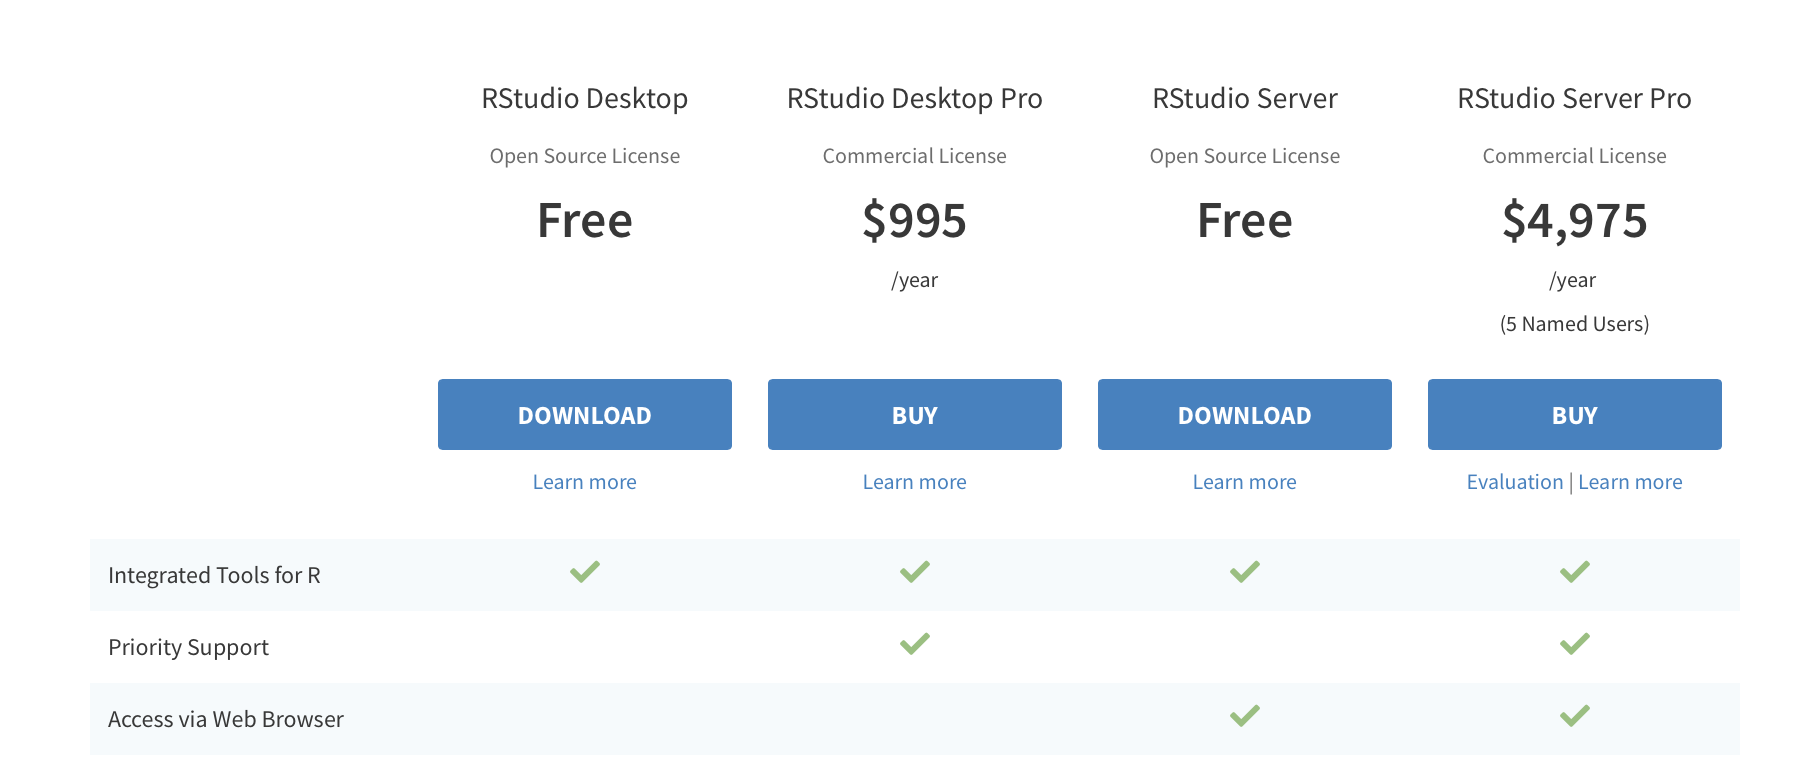
\includegraphics[width=0.8\linewidth]{C:/Data_Perso/theory_and_practice_of_field_experiments_french/Book/Images/new_rstudio} \caption{Sélectionner "Download" dans la colonne "RStudio Desktop Open Source License".}\label{fig:rstudiopng}
\end{figure}

\begin{figure}
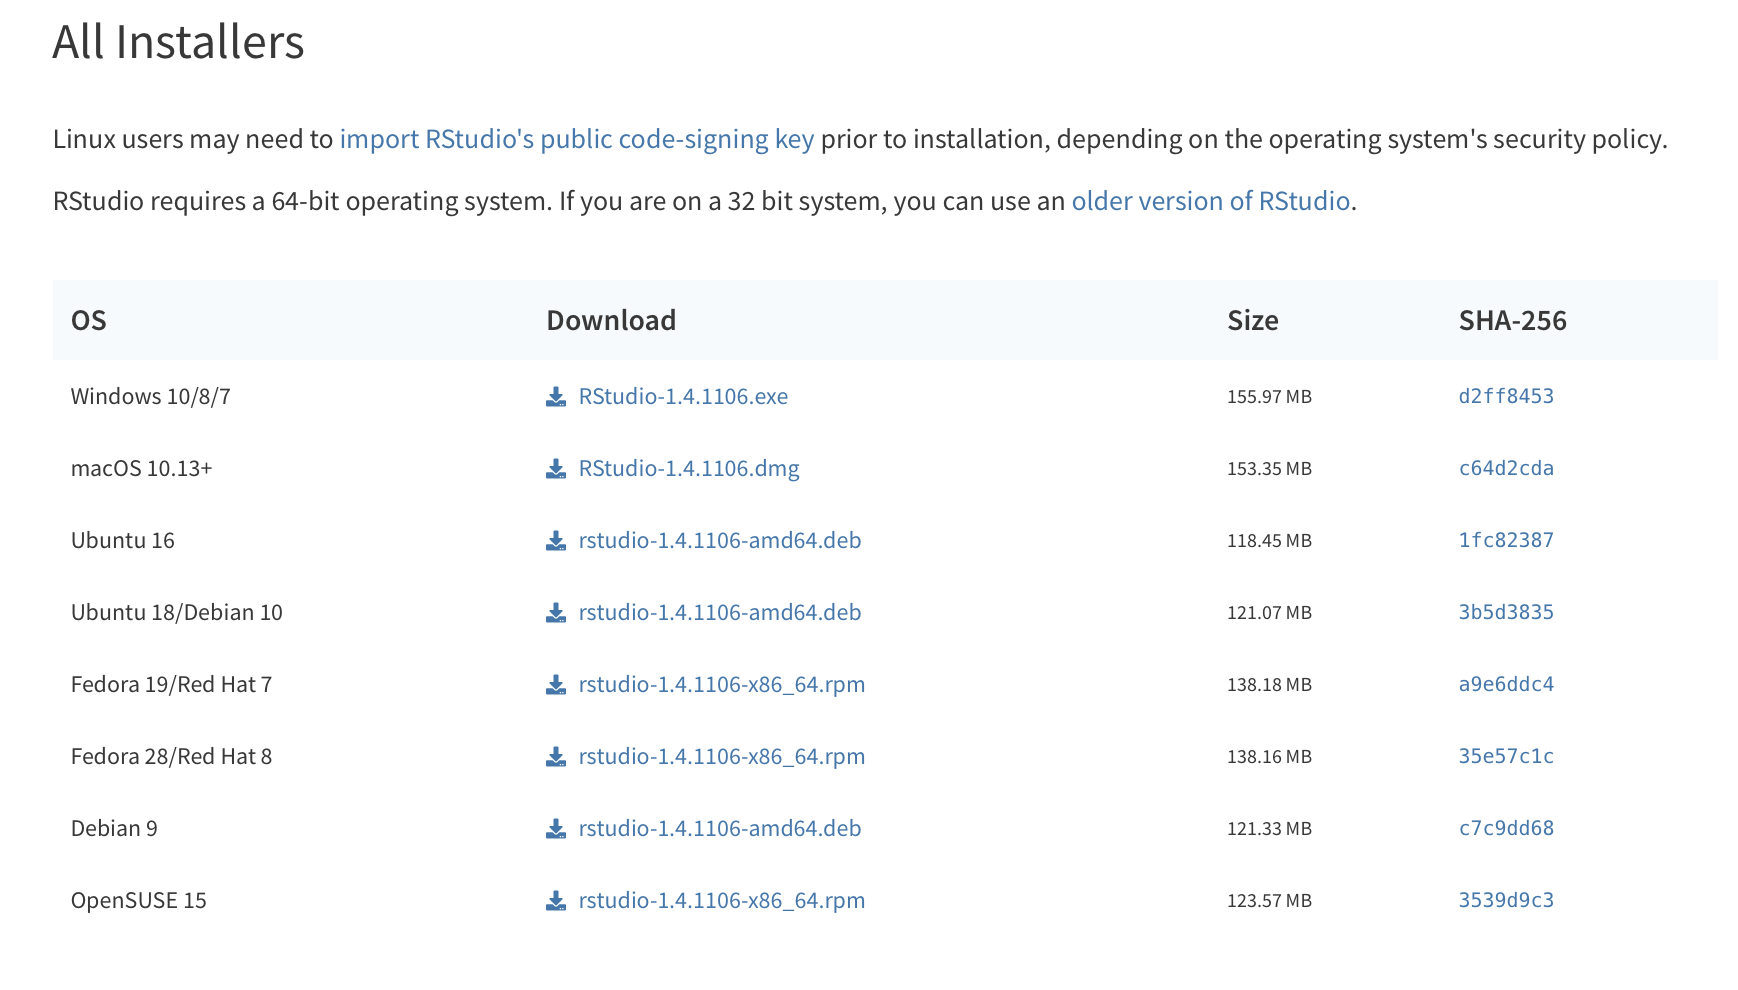
\includegraphics[width=0.8\linewidth]{Images/rstudio_download} \caption{Sélectionner le lien "Windows 10/8/7" pour Windows ou "Mac OS X 10.13+" pour Mac.}\label{fig:rstudiodownload}
\end{figure}

\hypertarget{linterface-rstudio}{%
\section{L'interface RStudio}\label{linterface-rstudio}}

Lorsque vous ouvrez RStudio pour la première fois, trois onglets doivent être visibles, comme illustré dans la Figure B.3 ci-dessous.

\begin{itemize}
\tightlist
\item
  Console (à gauche)
\item
  Accounting (en haut à droite) : cela inclue les onglets Environment et History
\item
  Miscellaneous (en bas à droite)
\end{itemize}

\begin{figure}
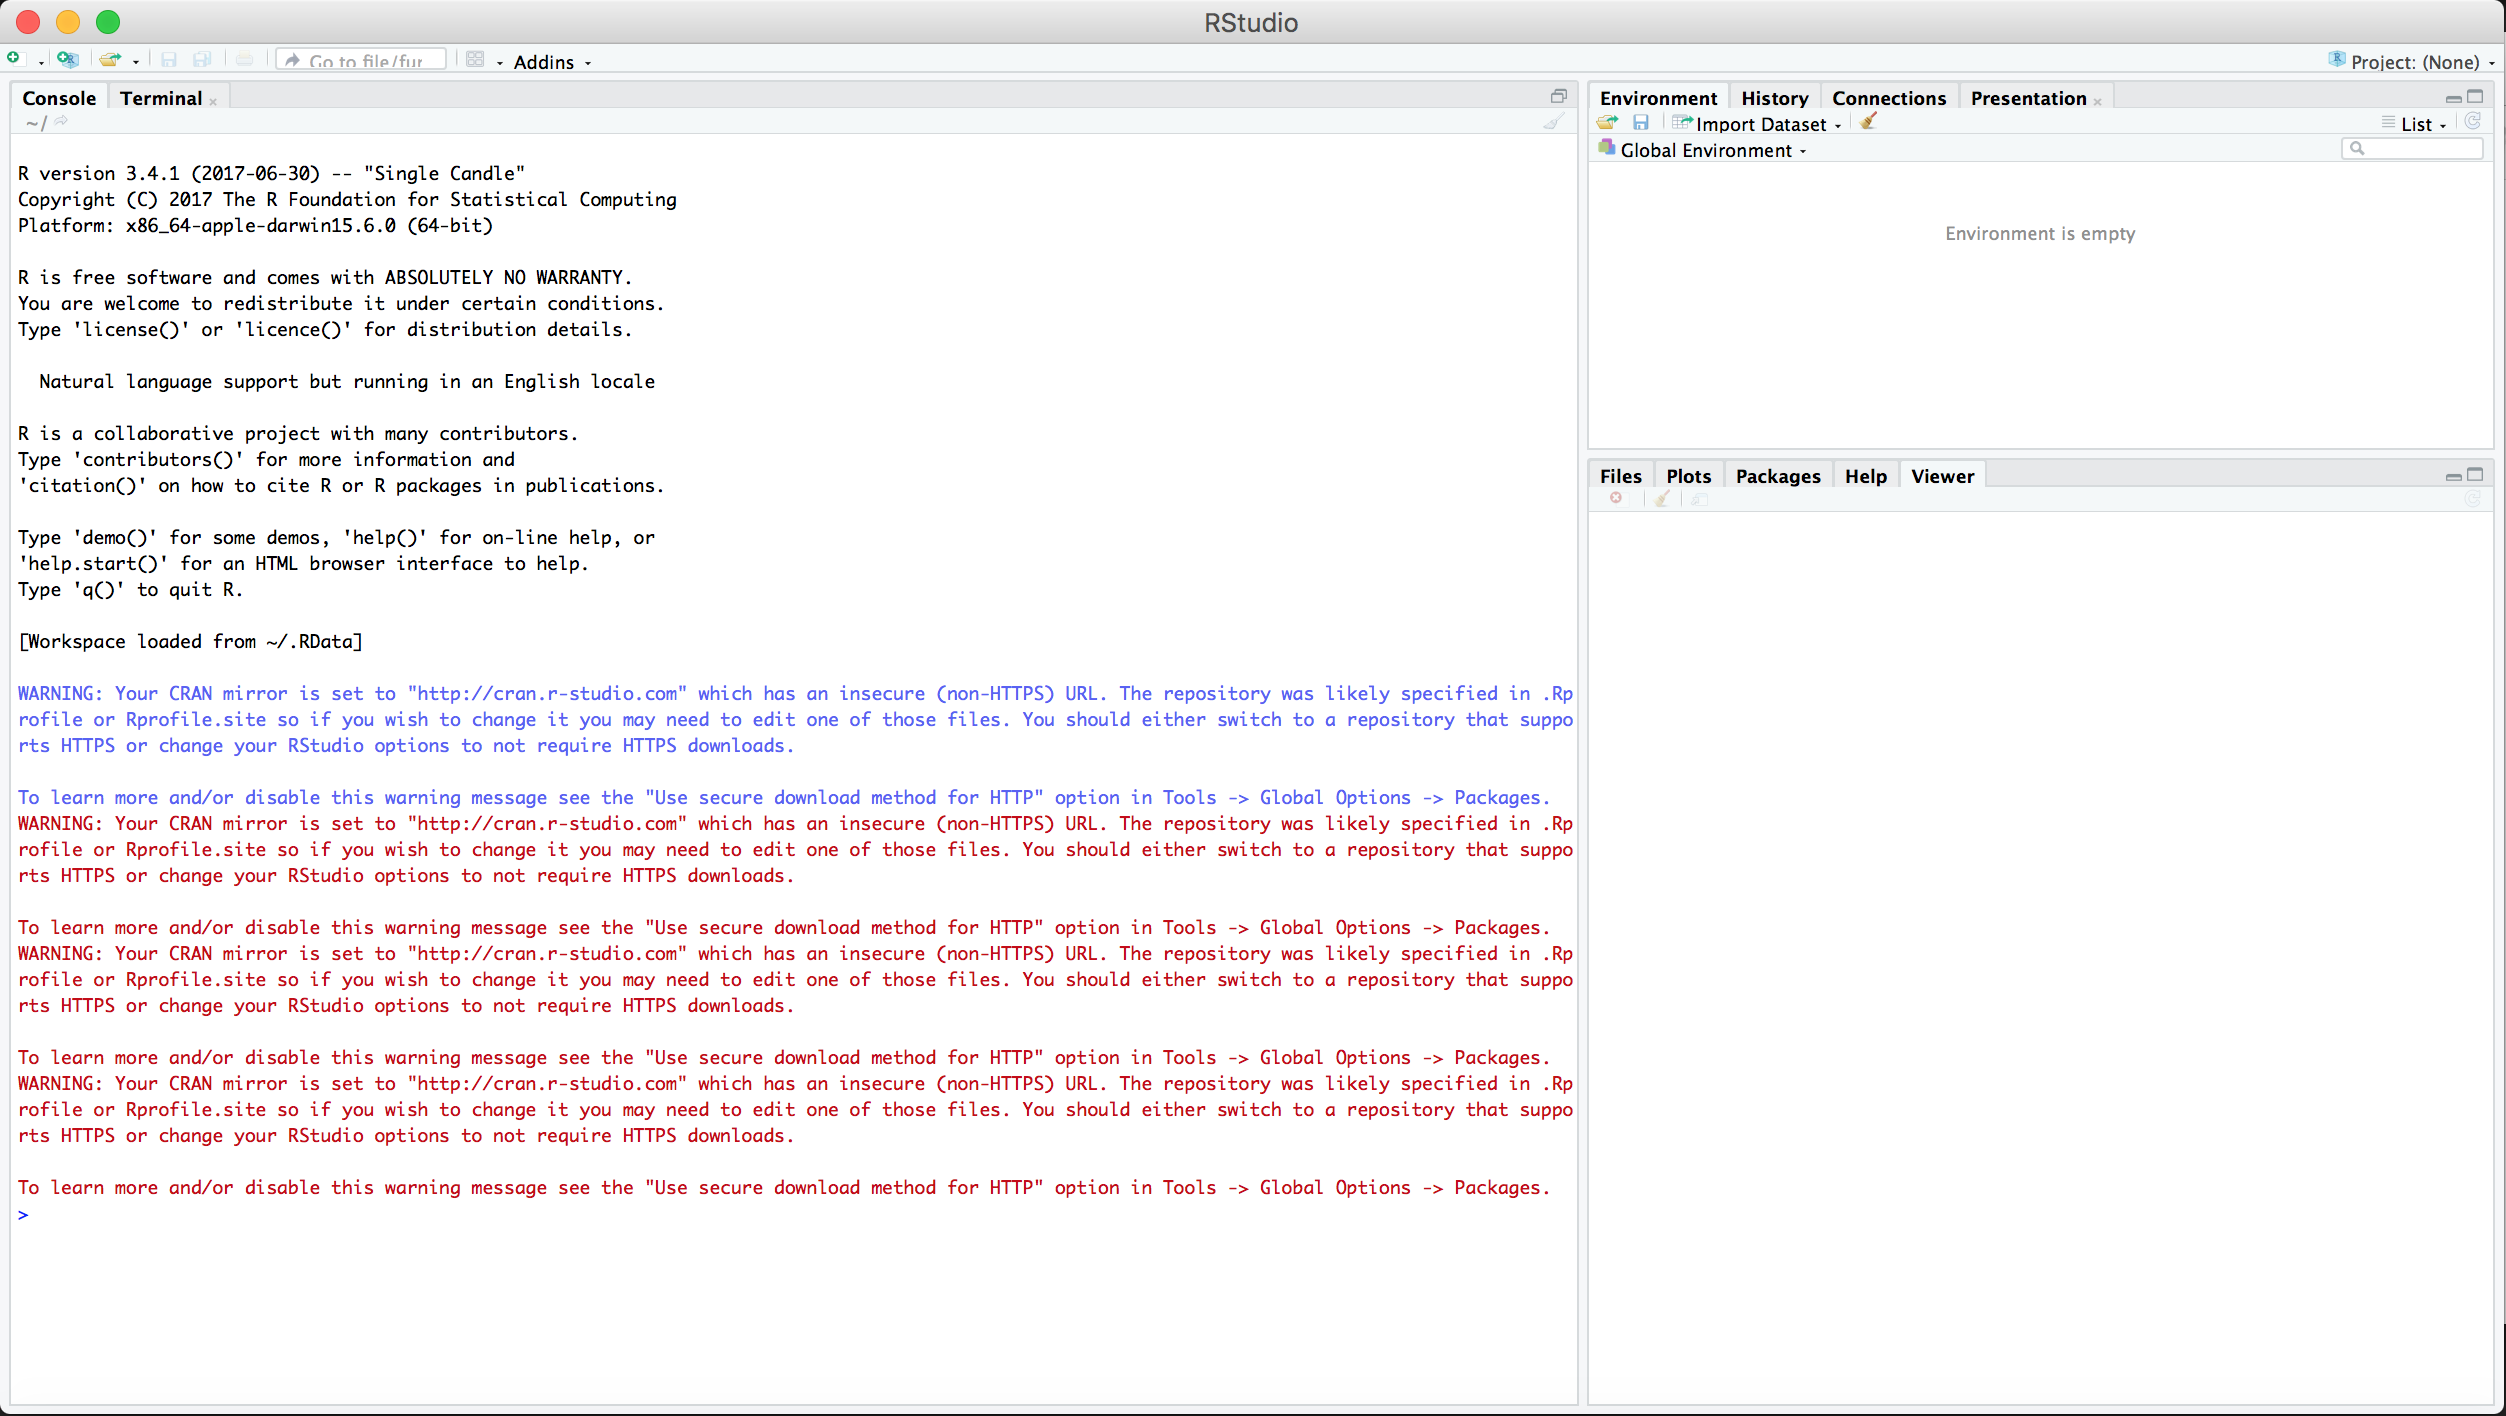
\includegraphics[width=0.8\linewidth]{Images/rstudio_intro} \caption{Lorsque vous ouvrez RStudio, il y a trois fenêtres visibles : la Console (à gauche), Accounting (en haut à droite), et Miscellaneous (en bas à droite).}\label{fig:rstudiointro}
\end{figure}

\hypertarget{la-console}{%
\subsection{La console}\label{la-console}}

Vous pouvez exécuter toutes les opérations dans la console. Par exemple, si vous saisissez \texttt{4\ +\ 4} et appuyez sur la touche Enter, la console renvoie \texttt{{[}1{]}\ 8}.

Pour s'assurer que tout le monde est prêt à utiliser R lors des Learning Days, nous demandons aux participants d'exécuter une ligne de code dans la console pour télécharger plusieurs packages R. Les packages sont des fragments de code reproducibles qui permettent une analyse plus efficace dans R. Pour exécuter ce bout de code, copiez-le dans la console et appuyez sur votre touche \texttt{Enter}. Vous devez être connecté à internet pour télécharger des packages.

\begin{Shaded}
\begin{Highlighting}[]
\FunctionTok{install.packages}\NormalTok{(}\FunctionTok{c}\NormalTok{(}
  \StringTok{"ggplot2"}\NormalTok{, }\StringTok{"dplyr"}\NormalTok{, }\StringTok{"AER"}\NormalTok{, }\StringTok{"arm"}\NormalTok{, }\StringTok{"MASS"}\NormalTok{, }\StringTok{"sandwich"}\NormalTok{,}
  \StringTok{"lmtest"}\NormalTok{, }\StringTok{"estimatr"}\NormalTok{, }\StringTok{"coin"}\NormalTok{, }\StringTok{"randomizr"}\NormalTok{, }\StringTok{"DeclareDesign"}
\NormalTok{))}
\end{Highlighting}
\end{Shaded}

Si le téléchargement est réussi, votre console ressemblera à la figure B.4, sauf que les URL seront différentes en fonction de votre emplacement.

\begin{figure}
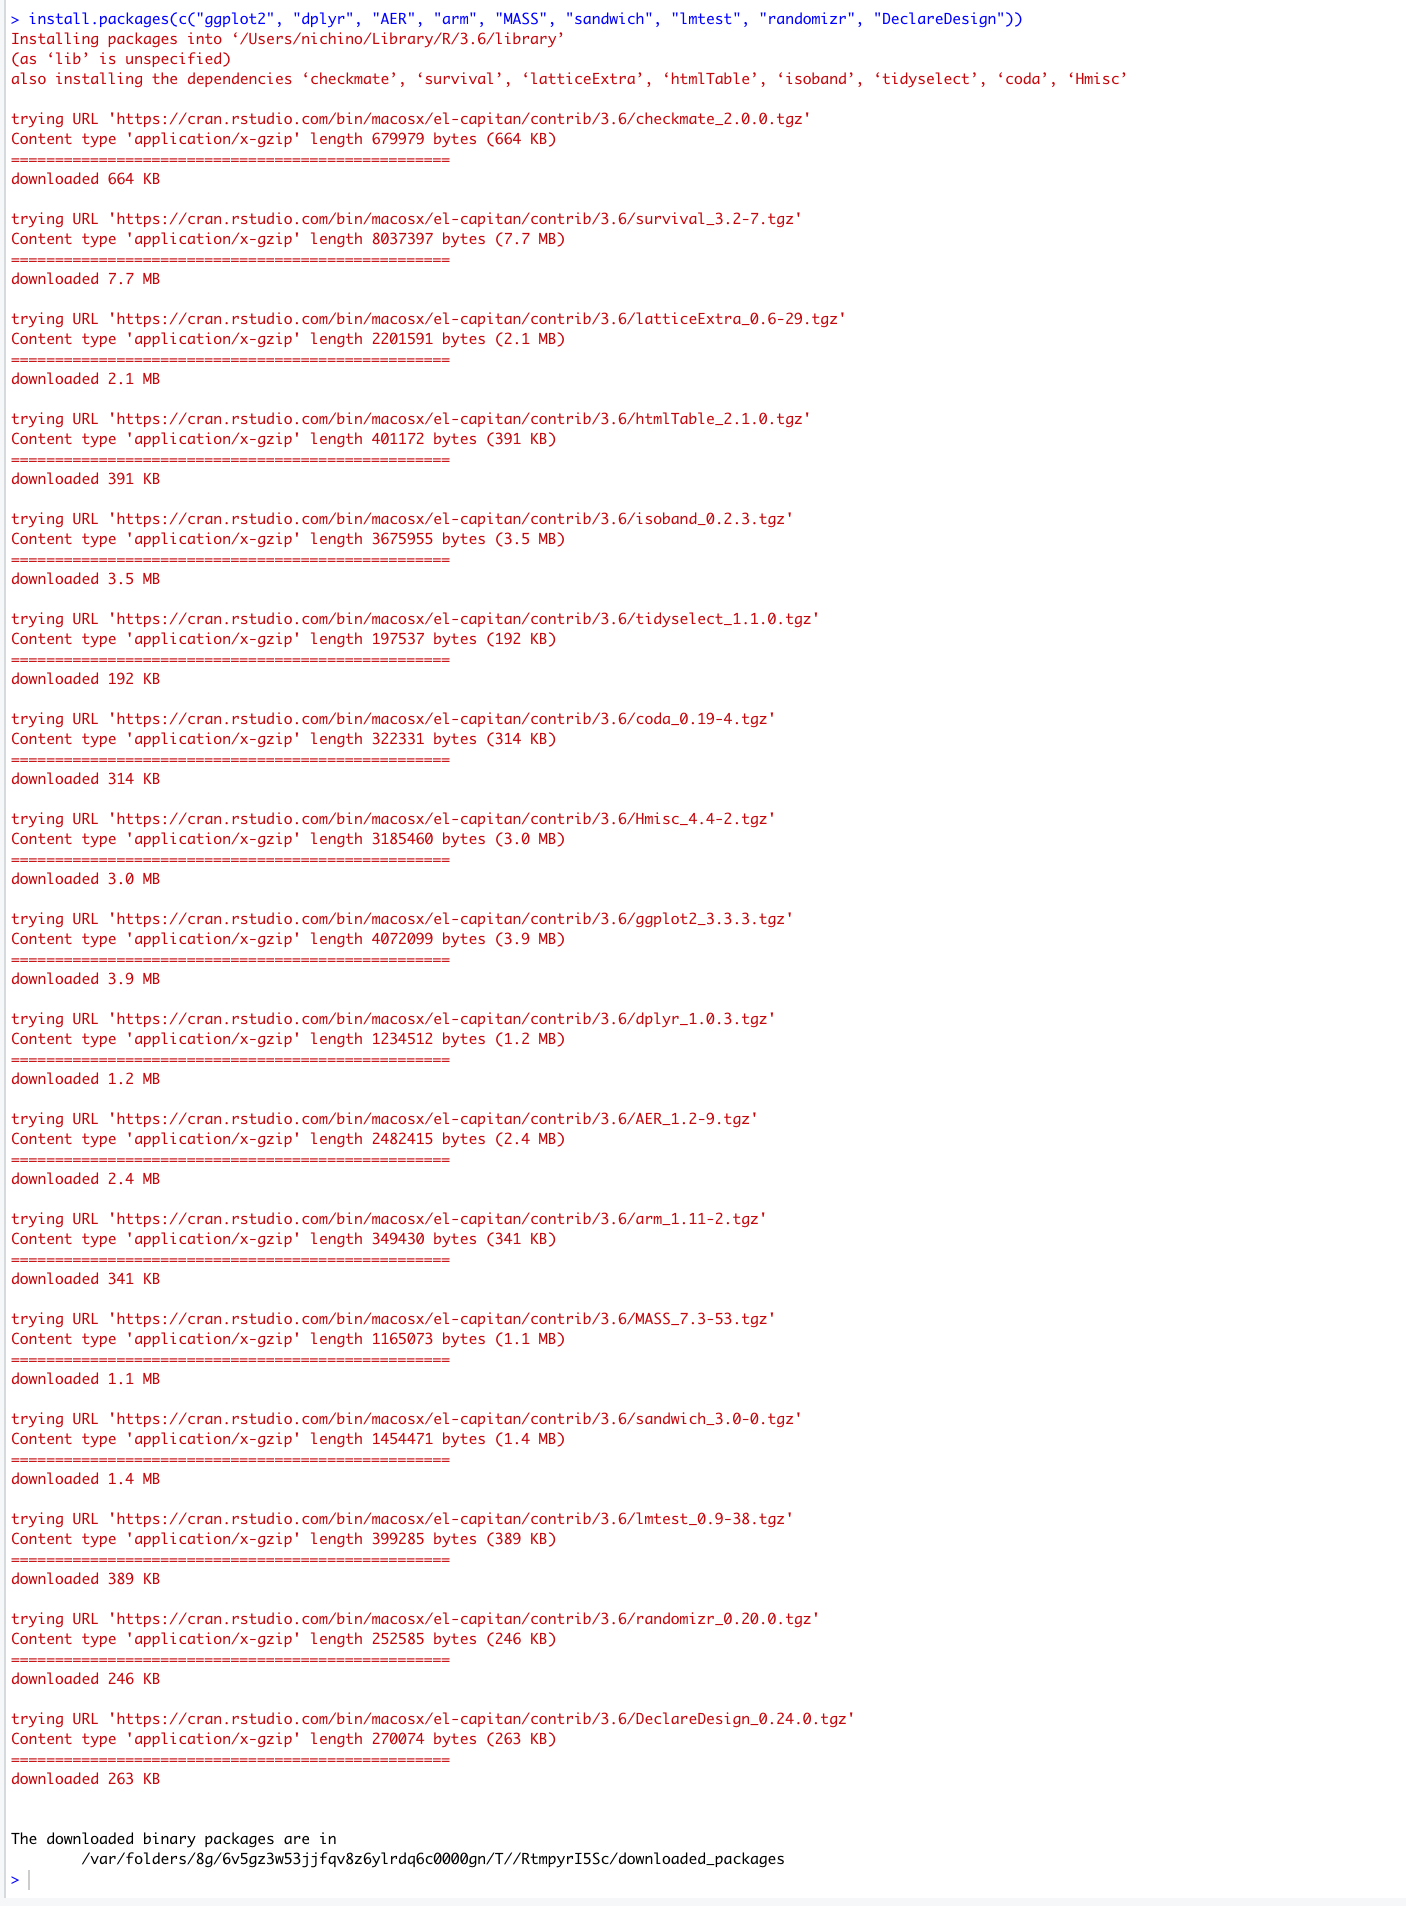
\includegraphics[width=0.4\linewidth]{Images/console2a} \caption{La console après avoir exécuté les trois lignes de code répertoriées ci-dessus.}\label{fig:console2}
\end{figure}

\hypertarget{luxe9diteur}{%
\subsection{L'éditeur}\label{luxe9diteur}}

Afin d'écrire et sauvegarder du code reproductible, nous allons ouvrir une quatrième fenêtre, l'éditeur, en cliquant sur l'icône avec une page blanche et un signe plus, dans le coin supérieur gauche de l'interface RStudio et en sélectionnant \texttt{R\ Script}, comme illustré à la figure B.5.

\begin{figure}
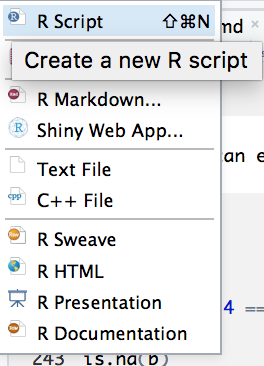
\includegraphics[width=0.6\linewidth]{Images/new_script} \caption{Créez un nouveau script R et ouvrez la fenêtre `éditeur` en sélectionnant `R Script` dans le menu déroulant.}\label{fig:newscript}
\end{figure}

Une fois le script R ouvert, il devrait y avoir quatre fenêtres dans l'interface RStudio, maintenant avec l'ajout de la fenêtre Éditeur. Nous pouvons exécuter une arithmétique simple en entrant une formule dans l'éditeur et en appuyant sur \texttt{Ctrl\ +\ Entrée} (Windows) ou \texttt{Commande\ +\ Entrée} (Mac). La formule et la ``réponse'' apparaîtront dans la console, comme illustré à la Figure B.6.

\begin{figure}
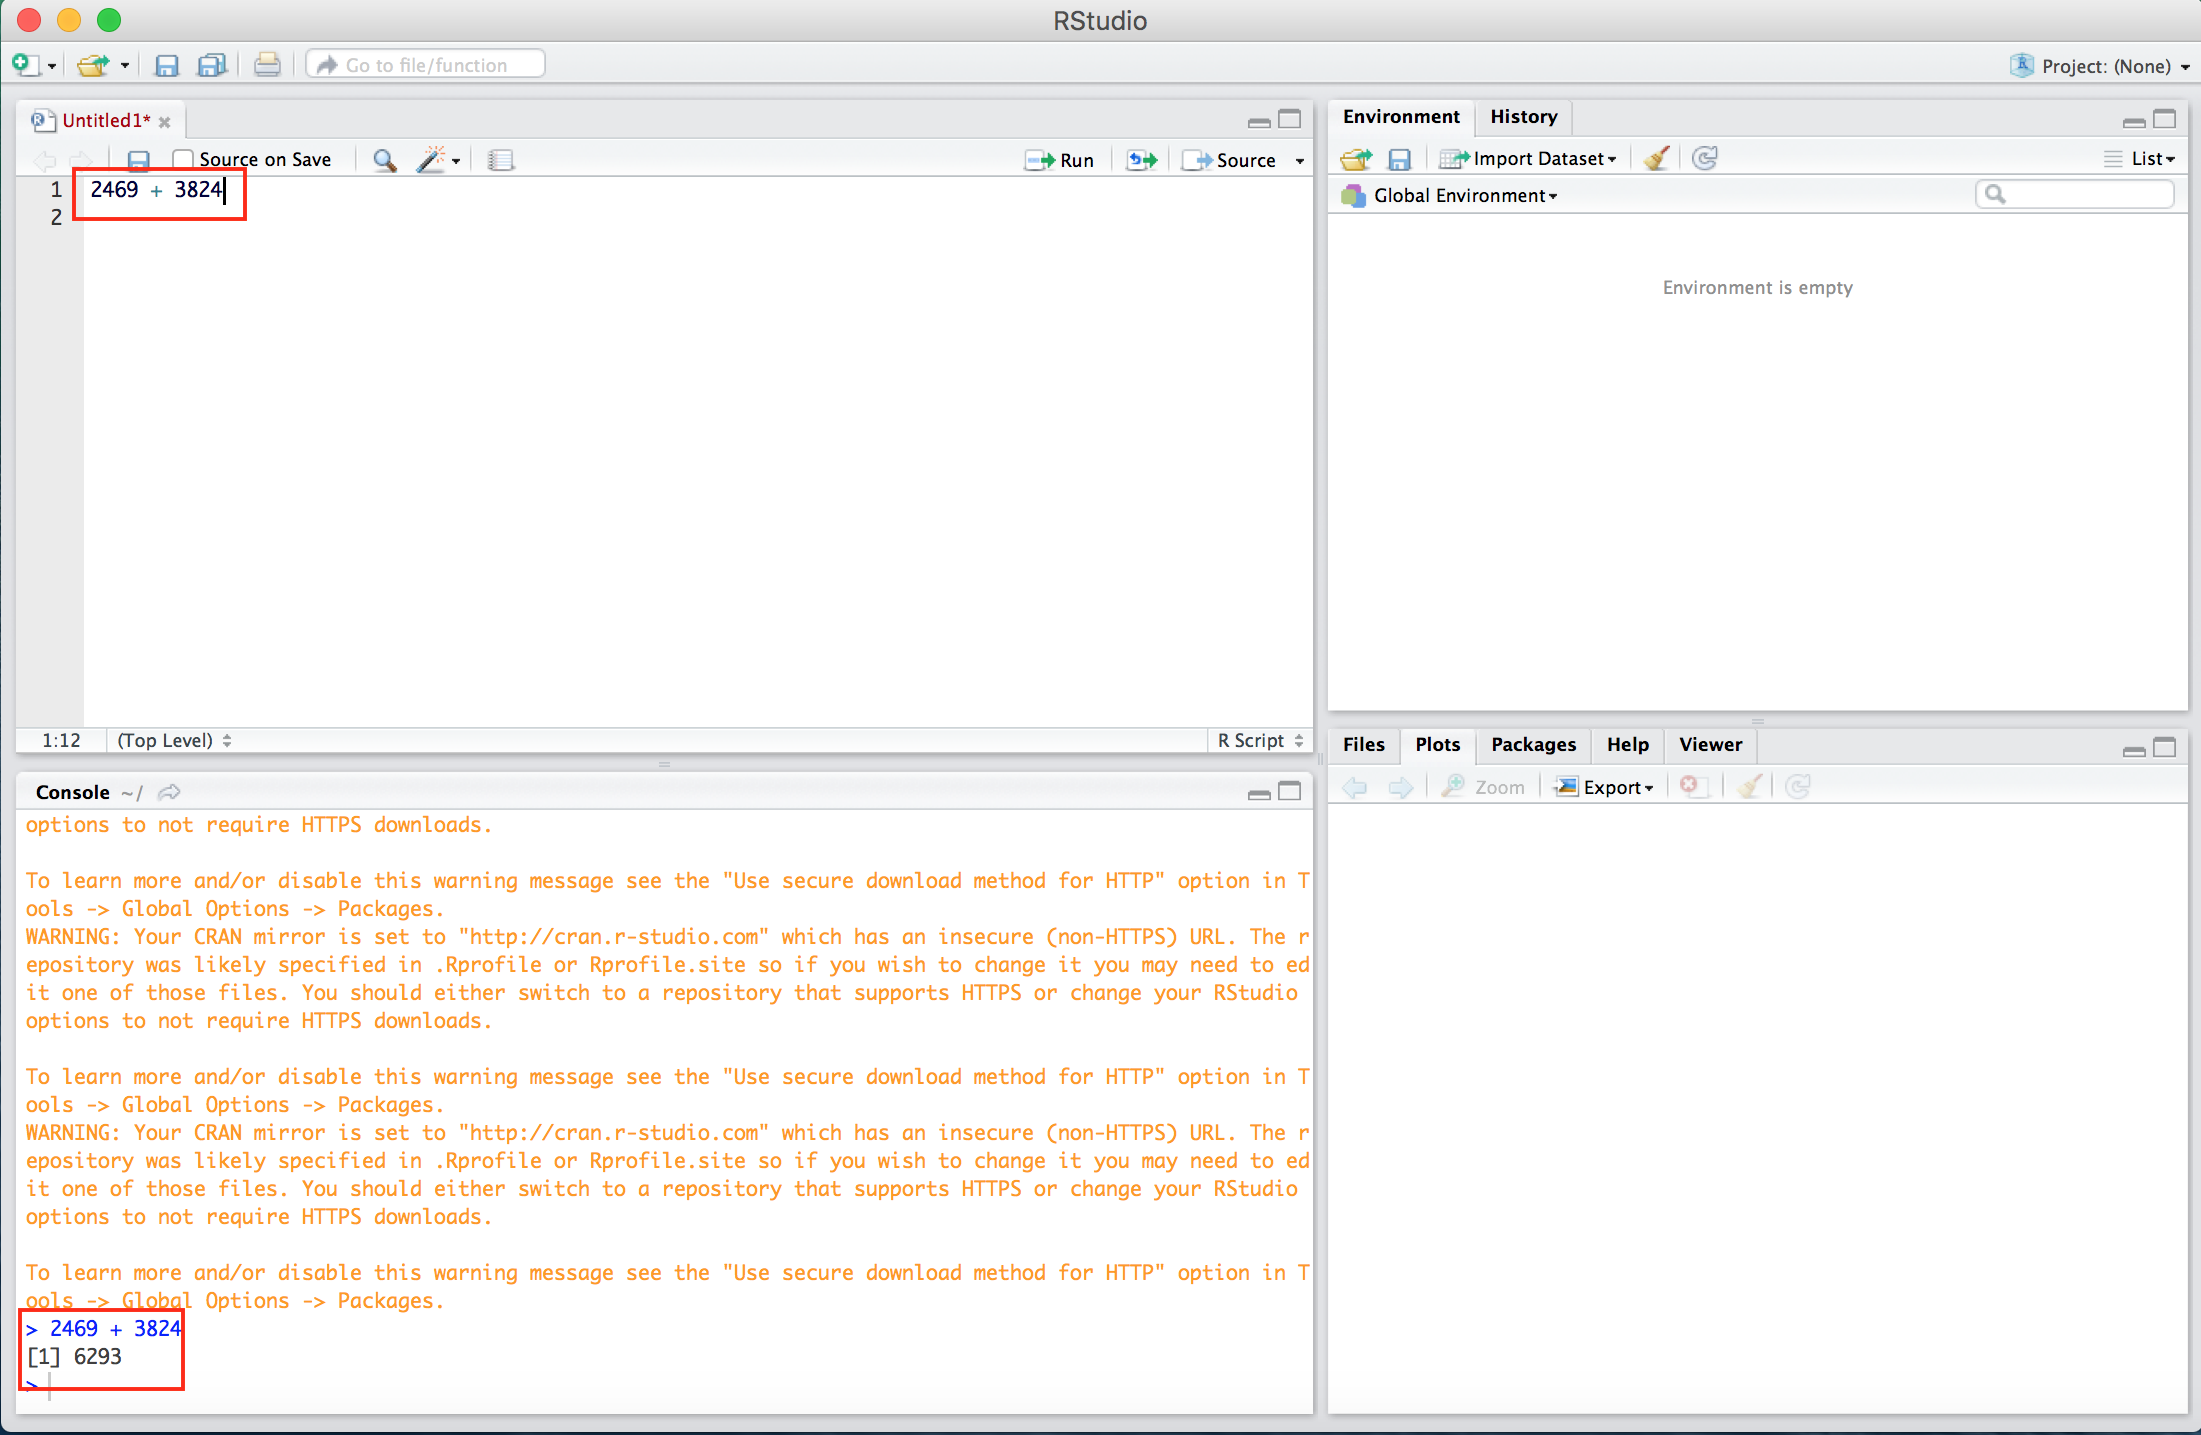
\includegraphics[width=0.6\linewidth]{Images/first_addition} \caption{Une expression arithmétique est saisie dans l'éditeur et évaluée dans la console. Les cases rouges sont ajoutées pour une visibilité accrue.}\label{fig:firstaddition}
\end{figure}

R peut être utilisé pour toute opération arithmétique, y compris, mais sans s'y limiter, l'addition (\texttt{+}), la soustraction (\texttt{-}), la multiplication scalaire (\texttt{*}), la division (\texttt{/}) et l'exponentielle (\texttt{\^{}} ).

\hypertarget{gestion}{%
\subsection{Gestion}\label{gestion}}

Au-delà des fonctions de base, nous pouvons également stocker des valeurs, des données et des fonctions dans l'environnement global. Pour affecter une valeur à une variable, utilisez l'opérateur \texttt{\textless{}-}. Toutes les valeurs, fonctions et données stockées apparaîtront dans l'onglet Environnement du fenêtre Gestion. Dans la Figure B.7, nous affectons la valeur \(3 \times \frac{6}{14}\) à la variable \texttt{t}, et pouvons voir qu'elle est stockée sous Valeurs.

Nous chargeons également un jeu de données. Ici, ``ChickWeight'' est un dataset intégré à R~; la plupart des datasets seront chargés à partir du Web ou d'autres fichiers sur votre ordinateur via une autre méthode. Nous pouvons voir que ChickWeight contient 578 observations de 4 variables et est stocké dans l'Environnement. En cliquant sur le nom ChickWeight, un onglet s'ouvrira avec le dataset dans la fenêtre de votre éditeur.

\begin{figure}
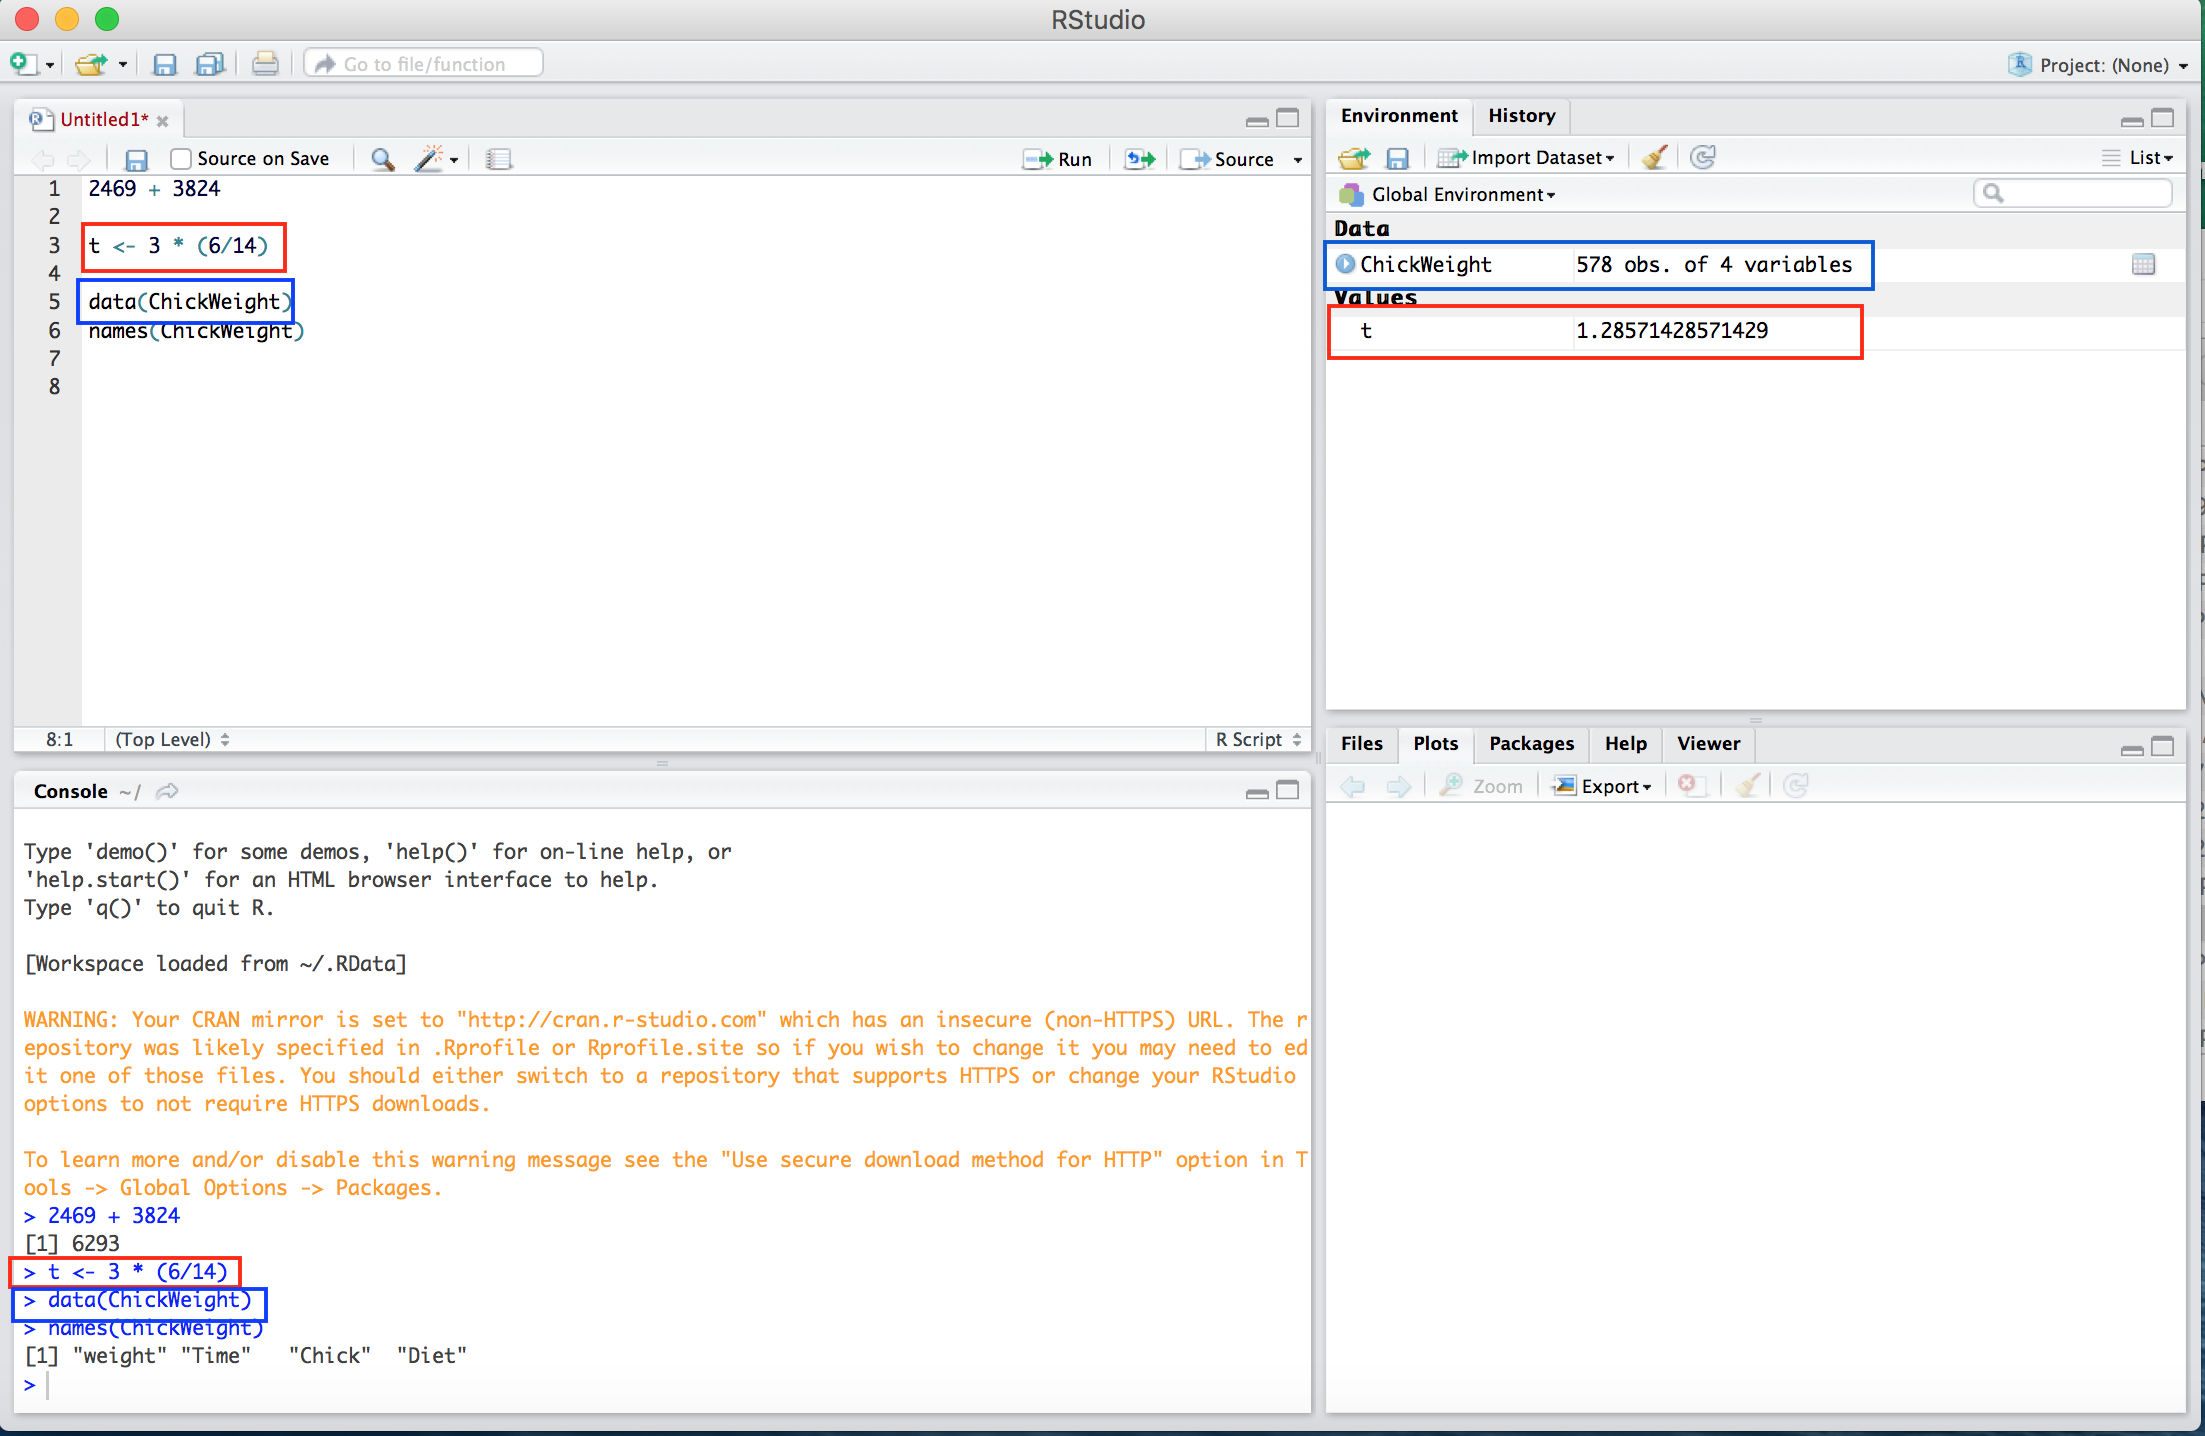
\includegraphics[width=0.6\linewidth]{Images/save_data} \caption{La valeur 3 * (6/14) est affectée à la variable t (en rouge) et le dataset ChickWeight est ajouté à l'environnement global (en bleu).}\label{fig:savedata}
\end{figure}

Les workshops Learning Days utilisent de nombreux outils dans R pour analyser et visualiser les données. Pour l'instant, nous pouvons apprendre quelques outils de base pour examiner les données. La fonction \texttt{head()} nous permet de voir les six premières lignes des données. \texttt{summary()} résume chacune des colonnes du dataset et \texttt{dim()} fournit les dimensions du dataset avec d'abord le nombre de lignes puis de colonnes.

\begin{Shaded}
\begin{Highlighting}[]
\FunctionTok{head}\NormalTok{(ChickWeight) }\CommentTok{\# Les 6 premières observations du dataset}
\end{Highlighting}
\end{Shaded}

\begin{verbatim}
  weight Time Chick Diet
1     42    0     1    1
2     51    2     1    1
3     59    4     1    1
4     64    6     1    1
5     76    8     1    1
6     93   10     1    1
\end{verbatim}

\begin{Shaded}
\begin{Highlighting}[]
\FunctionTok{summary}\NormalTok{(ChickWeight) }\CommentTok{\# Résumé de toutes les variables}
\end{Highlighting}
\end{Shaded}

\begin{verbatim}
     weight         Time          Chick     Diet   
 Min.   : 35   Min.   : 0.0   13     : 12   1:220  
 1st Qu.: 63   1st Qu.: 4.0   9      : 12   2:120  
 Median :103   Median :10.0   20     : 12   3:120  
 Mean   :122   Mean   :10.7   10     : 12   4:118  
 3rd Qu.:164   3rd Qu.:16.0   17     : 12          
 Max.   :373   Max.   :21.0   19     : 12          
                              (Other):506          
\end{verbatim}

\begin{Shaded}
\begin{Highlighting}[]
\FunctionTok{dim}\NormalTok{(ChickWeight) }\CommentTok{\# Dimensions du dataset dans l\textquotesingle{}ordre "ligne" puis "colonne"}
\end{Highlighting}
\end{Shaded}

\begin{verbatim}
[1] 578   4
\end{verbatim}

Contrairement à d'autres logiciels statistiques, R permet aux utilisateurs de stocker simultanément plusieurs ensembles de données, éventuellement de dimensions différentes. Cette fonctionnalité rend R assez flexible pour l'analyse à l'aide de plusieurs méthodes.

\hypertarget{divers}{%
\subsection{Divers}\label{divers}}

R fournit une suite d'outils, allant des fonctions intégrées aux packages pour tracer graphiques, modèles, estimations, etc. La dernière fenêtre Divers permet une visualisation rapide des graphiques dans RStudio. La Figure B.8 montre une courbe dans cette fenêtre. Pendant les Leaning Days, on discutera de la manière de représenter les données.

\begin{figure}
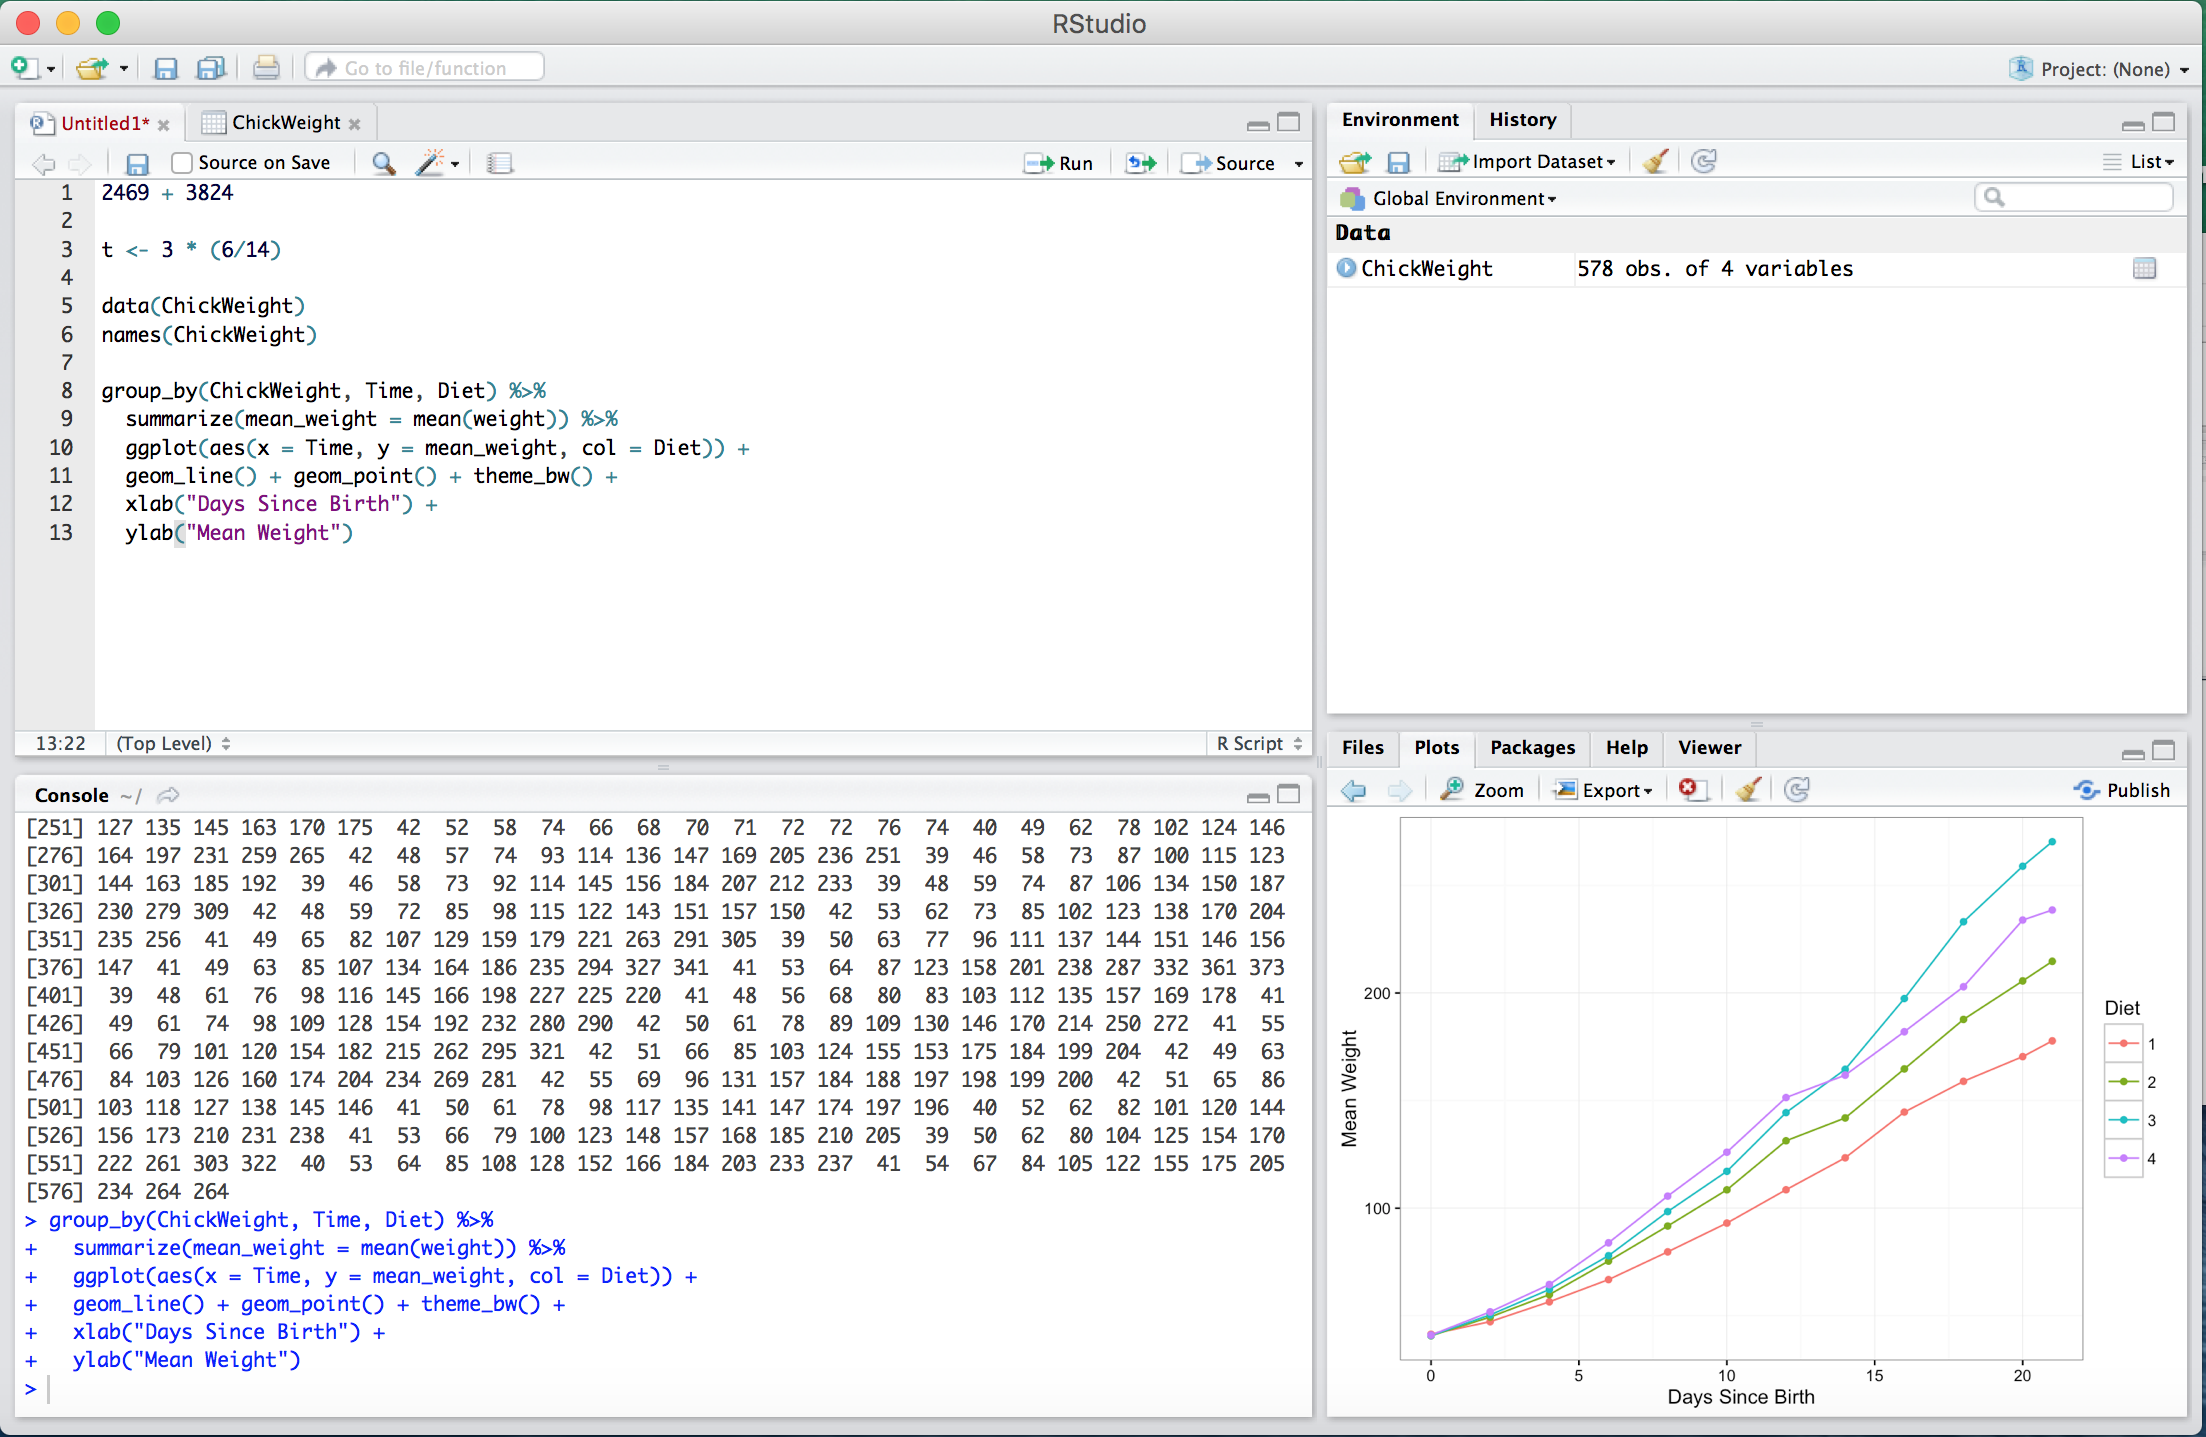
\includegraphics[width=0.6\linewidth]{Images/graph} \caption{Un exemple de courbe avec le dataset `ChickWeight` en R.}\label{fig:graph}
\end{figure}

\hypertarget{apprendre-uxe0-utiliser-r}{%
\section{Apprendre à utiliser R}\label{apprendre-uxe0-utiliser-r}}

\hypertarget{ressources-en-ligne}{%
\subsection{Ressources en ligne}\label{ressources-en-ligne}}

Il existe de nombreuses ressources en ligne utiles pour vous aider à commencer avec R. Nous vous recommandons deux sources~:

\begin{itemize}
\tightlist
\item
  Code School, qui fonctionne entièrement sur votre navigateur \url{https://www.codeschool.com/courses/try-r}.
\item
  Coursera, via un cours de programmation R en ligne organisé par l'Université Johns Hopkins :

  \begin{enumerate}
  \def\labelenumi{\roman{enumi}.}
  \tightlist
  \item
    Allez sur \url{https://www.coursera.org}
  \item
    Créez un compte (c'est gratuit !)
  \item
    Inscrivez-vous pour ``R Programming at Johns Hopkins University'' (instructeur : Roger Peng) sous la rubrique ``Cours''
  \item
    Lisez les documents et regardez les vidéos de la première semaine. Les vidéos de la première semaine durent environ 2 heures 30 au total.
  \end{enumerate}
\end{itemize}

\hypertarget{exercise-de-base}{%
\subsection{Exercise de base}\label{exercise-de-base}}

Voici quelques fragments de code pour vous familiariser avec certaines pratiques de base de R. Nous vous recommandons de vous entraîner en tapant les fragments de code dans votre éditeur, puis en les évaluant.

\hypertarget{configuration-dune-session-r}{%
\subsubsection{Configuration d'une session R}\label{configuration-dune-session-r}}

En général, nous lisons d'autres fichiers tels que des données ou des fonctions dans R et publions des résultats tels que des graphiques ou des tableaux dans des fichiers en dehors de la session R. Pour ce faire, nous devons donner à R une ``adresse'' où il peut localiser de tels fichiers. Il peut être plus efficace de le faire en définissant un répertoire de travail, i.e.~un chemin d'accès au répertoire dans lequel les fichiers pertinents sont stockés. Nous pouvons identifier le répertoire de travail actuel en utilisant \texttt{getwd()} et le définir en utilisant \texttt{setwd()}. Notez que la syntaxe de ces chemins de fichiers varie selon le système d'exploitation.

\begin{Shaded}
\begin{Highlighting}[]
\FunctionTok{getwd}\NormalTok{()}
\end{Highlighting}
\end{Shaded}

\begin{Shaded}
\begin{Highlighting}[]
\FunctionTok{setwd}\NormalTok{(}\StringTok{"\textasciitilde{}TaraLyn/EGAP Learning Days Admin/Workshop 2018\_2 (Uruguay)/"}\NormalTok{)}
\end{Highlighting}
\end{Shaded}

Vous devrez peut-être installer des packages autres que ceux répertoriés ci-dessus pour exécuter certaines fonctions. Pour installer les packages, nous utilisons \texttt{install.packages("")}, en remplissant le nom du package entre les marques "", comme suit. Vous n'avez besoin d'installer les packages qu'une seule fois.

\begin{Shaded}
\begin{Highlighting}[]
\FunctionTok{install.packages}\NormalTok{(}\StringTok{"randomizr"}\NormalTok{)}
\end{Highlighting}
\end{Shaded}

Une fois qu'un package est installé, il peut être chargé et accessible en utilisant \texttt{library()} où le nom du package est inséré entre parenthèses (sans guillemets).

\begin{Shaded}
\begin{Highlighting}[]
\FunctionTok{library}\NormalTok{(randomizr)}
\end{Highlighting}
\end{Shaded}

Pour effacer de la mémoire de R, les données, fonctions ou valeurs stockées qui apparaissent dans l'onglet de comptabilité, utilisez \texttt{rm(list\ =\ ls())}. Il peut être utile de définir un nombre aléatoire pour garantir que la réplication est possible dans une session R différente, en particulier lorsque nous travaillons avec des méthodes basées sur la simulation.

\begin{Shaded}
\begin{Highlighting}[]
\FunctionTok{rm}\NormalTok{(}\AttributeTok{list =} \FunctionTok{ls}\NormalTok{())}
\FunctionTok{set.seed}\NormalTok{(}\DecValTok{2018}\NormalTok{) }\CommentTok{\# pour la reproductibilité}
\end{Highlighting}
\end{Shaded}

\hypertarget{les-basiques}{%
\subsubsection{Les basiques}\label{les-basiques}}

Nous allons maintenant explorer quelques commandes de base. Afin d'affecter un scalaire (i.e.~un élément unique) à une variable, nous utilisons la commande \texttt{\textless{}-} comme discuté précédemment :

\begin{Shaded}
\begin{Highlighting}[]
\CommentTok{\# "\textless{}{-}"  est la commande d\textquotesingle{}affectation ; ça sert à définir les choses. eg :}
\NormalTok{(a }\OtherTok{\textless{}{-}} \DecValTok{5}\NormalTok{)}
\end{Highlighting}
\end{Shaded}

\begin{verbatim}
[1] 5
\end{verbatim}

Nous pouvons également vouloir affecter un vecteur d'éléments à une variable. Ici, nous utilisons la même commande \texttt{\textless{}-}, mais nous nous concentrons sur la façon de créer le vecteur.

\begin{Shaded}
\begin{Highlighting}[]
\CommentTok{\# ":"  est utilisé pour définir une chaîne d\textquotesingle{}entiers}
\NormalTok{(b }\OtherTok{\textless{}{-}} \DecValTok{1}\SpecialCharTok{:}\DecValTok{10}\NormalTok{)}
\end{Highlighting}
\end{Shaded}

\begin{verbatim}
 [1]  1  2  3  4  5  6  7  8  9 10
\end{verbatim}

\begin{Shaded}
\begin{Highlighting}[]
\CommentTok{\# utilisez c() pour faire un vecteur avec n\textquotesingle{}importe quoi dedans}
\NormalTok{(v }\OtherTok{\textless{}{-}} \FunctionTok{c}\NormalTok{(}\DecValTok{1}\NormalTok{, }\DecValTok{3}\NormalTok{, }\DecValTok{2}\NormalTok{, }\DecValTok{4}\NormalTok{, pi))}
\end{Highlighting}
\end{Shaded}

\begin{verbatim}
[1] 1.000 3.000 2.000 4.000 3.142
\end{verbatim}

On peut alors se référer aux éléments d'un vecteur en désignant leur position à l'intérieur de parenthèses \texttt{{[}{]}}.

\begin{Shaded}
\begin{Highlighting}[]
\CommentTok{\# Extrait les éléments d\textquotesingle{}un vecteur :}
\NormalTok{b[}\DecValTok{1}\NormalTok{] }\CommentTok{\# Retourne la position 1}
\end{Highlighting}
\end{Shaded}

\begin{verbatim}
[1] 1
\end{verbatim}

\begin{Shaded}
\begin{Highlighting}[]
\NormalTok{b[}\DecValTok{5}\SpecialCharTok{:}\DecValTok{4}\NormalTok{] }\CommentTok{\# Retourne les positions 5 et 4, dans cet ordre}
\end{Highlighting}
\end{Shaded}

\begin{verbatim}
[1] 5 4
\end{verbatim}

\begin{Shaded}
\begin{Highlighting}[]
\NormalTok{b[}\SpecialCharTok{{-}}\DecValTok{1}\NormalTok{] }\CommentTok{\# Retourne tout sauf le premier élément}
\end{Highlighting}
\end{Shaded}

\begin{verbatim}
[1]  2  3  4  5  6  7  8  9 10
\end{verbatim}

\begin{Shaded}
\begin{Highlighting}[]
\CommentTok{\# Retourne tous les nombres indiqués comme "TRUE"}
\NormalTok{b[}\FunctionTok{c}\NormalTok{(}\ConstantTok{TRUE}\NormalTok{, }\ConstantTok{FALSE}\NormalTok{, }\ConstantTok{TRUE}\NormalTok{, }\ConstantTok{FALSE}\NormalTok{, }\ConstantTok{FALSE}\NormalTok{, }\ConstantTok{TRUE}\NormalTok{, }\ConstantTok{TRUE}\NormalTok{, }\ConstantTok{FALSE}\NormalTok{, }\ConstantTok{FALSE}\NormalTok{, }\ConstantTok{FALSE}\NormalTok{)]}
\end{Highlighting}
\end{Shaded}

\begin{verbatim}
[1] 1 3 6 7
\end{verbatim}

\begin{Shaded}
\begin{Highlighting}[]
\CommentTok{\# Attribue une nouvelle valeur à l\textquotesingle{}élément particulier d\textquotesingle{}un vecteur}
\NormalTok{b[}\DecValTok{5}\NormalTok{] }\OtherTok{\textless{}{-}} \DecValTok{0}
\end{Highlighting}
\end{Shaded}

Il existe un ensemble de fonctions pré-existantes qui peuvent être appliquées à des vecteurs comme \texttt{b}.

\begin{Shaded}
\begin{Highlighting}[]
\FunctionTok{sum}\NormalTok{(b) }\CommentTok{\# Somme de tous les éléments}
\end{Highlighting}
\end{Shaded}

\begin{verbatim}
[1] 50
\end{verbatim}

\begin{Shaded}
\begin{Highlighting}[]
\FunctionTok{mean}\NormalTok{(b) }\CommentTok{\# Moyenne de tous les éléments}
\end{Highlighting}
\end{Shaded}

\begin{verbatim}
[1] 5
\end{verbatim}

\begin{Shaded}
\begin{Highlighting}[]
\FunctionTok{max}\NormalTok{(b) }\CommentTok{\# Maximum de tous les éléments}
\end{Highlighting}
\end{Shaded}

\begin{verbatim}
[1] 10
\end{verbatim}

\begin{Shaded}
\begin{Highlighting}[]
\FunctionTok{min}\NormalTok{(b) }\CommentTok{\# Minimum de tous les éléments}
\end{Highlighting}
\end{Shaded}

\begin{verbatim}
[1] 0
\end{verbatim}

\begin{Shaded}
\begin{Highlighting}[]
\FunctionTok{sd}\NormalTok{(b) }\CommentTok{\# Écart type de tous les éléments}
\end{Highlighting}
\end{Shaded}

\begin{verbatim}
[1] 3.496
\end{verbatim}

\begin{Shaded}
\begin{Highlighting}[]
\FunctionTok{var}\NormalTok{(b) }\CommentTok{\# Variance de tous les éléments}
\end{Highlighting}
\end{Shaded}

\begin{verbatim}
[1] 12.22
\end{verbatim}

On peut aussi appliquer des transformations arithmétiques à tous les éléments d'un vecteur :

\begin{Shaded}
\begin{Highlighting}[]
\NormalTok{b}\SpecialCharTok{\^{}}\DecValTok{2} \CommentTok{\# Carré de la variable}
\end{Highlighting}
\end{Shaded}

\begin{verbatim}
 [1]   1   4   9  16   0  36  49  64  81 100
\end{verbatim}

\begin{Shaded}
\begin{Highlighting}[]
\NormalTok{b}\SpecialCharTok{\^{}}\NormalTok{.}\DecValTok{5} \CommentTok{\# Racine carré de la variable}
\end{Highlighting}
\end{Shaded}

\begin{verbatim}
 [1] 1.000 1.414 1.732 2.000 0.000 2.449 2.646 2.828 3.000 3.162
\end{verbatim}

\begin{Shaded}
\begin{Highlighting}[]
\FunctionTok{log}\NormalTok{(b) }\CommentTok{\# Log de la variable}
\end{Highlighting}
\end{Shaded}

\begin{verbatim}
 [1] 0.0000 0.6931 1.0986 1.3863   -Inf 1.7918 1.9459 2.0794 2.1972 2.3026
\end{verbatim}

\begin{Shaded}
\begin{Highlighting}[]
\FunctionTok{exp}\NormalTok{(b) }\CommentTok{\# Exponentielle de la variable}
\end{Highlighting}
\end{Shaded}

\begin{verbatim}
 [1]     2.718     7.389    20.086    54.598     1.000   403.429  1096.633  2980.958  8103.084 22026.466
\end{verbatim}

Enfin, nous pouvons évaluer les affirmations logiques (c'est-à-dire ``la condition X est-elle vraie~?'') sur tous les éléments d'un vecteur :

\begin{Shaded}
\begin{Highlighting}[]
\NormalTok{b }\SpecialCharTok{==} \DecValTok{2} \CommentTok{\# égal à}
\end{Highlighting}
\end{Shaded}

\begin{verbatim}
 [1] FALSE  TRUE FALSE FALSE FALSE FALSE FALSE FALSE FALSE FALSE
\end{verbatim}

\begin{Shaded}
\begin{Highlighting}[]
\NormalTok{b }\SpecialCharTok{\textless{}} \DecValTok{5} \CommentTok{\# plus petit que}
\end{Highlighting}
\end{Shaded}

\begin{verbatim}
 [1]  TRUE  TRUE  TRUE  TRUE  TRUE FALSE FALSE FALSE FALSE FALSE
\end{verbatim}

\begin{Shaded}
\begin{Highlighting}[]
\NormalTok{b }\SpecialCharTok{\textgreater{}=} \DecValTok{5} \CommentTok{\# plus petit ou égal à}
\end{Highlighting}
\end{Shaded}

\begin{verbatim}
 [1] FALSE FALSE FALSE FALSE FALSE  TRUE  TRUE  TRUE  TRUE  TRUE
\end{verbatim}

\begin{Shaded}
\begin{Highlighting}[]
\NormalTok{b }\SpecialCharTok{\textless{}=} \DecValTok{5} \SpecialCharTok{|}\NormalTok{ b }\SpecialCharTok{/} \DecValTok{4} \SpecialCharTok{==} \DecValTok{2} \CommentTok{\# | signifie OU}
\end{Highlighting}
\end{Shaded}

\begin{verbatim}
 [1]  TRUE  TRUE  TRUE  TRUE  TRUE FALSE FALSE  TRUE FALSE FALSE
\end{verbatim}

\begin{Shaded}
\begin{Highlighting}[]
\NormalTok{b }\SpecialCharTok{\textgreater{}} \DecValTok{2} \SpecialCharTok{\&}\NormalTok{ b }\SpecialCharTok{\textless{}} \DecValTok{9} \CommentTok{\# \& signifie ET}
\end{Highlighting}
\end{Shaded}

\begin{verbatim}
 [1] FALSE FALSE  TRUE  TRUE FALSE  TRUE  TRUE  TRUE FALSE FALSE
\end{verbatim}

\begin{Shaded}
\begin{Highlighting}[]
\FunctionTok{is.na}\NormalTok{(b) }\CommentTok{\# Indique si la donnée est manquante}
\end{Highlighting}
\end{Shaded}

\begin{verbatim}
 [1] FALSE FALSE FALSE FALSE FALSE FALSE FALSE FALSE FALSE FALSE
\end{verbatim}

\begin{Shaded}
\begin{Highlighting}[]
\CommentTok{\# Donne les indices des éléments dont la valeur répond à la condition}
\FunctionTok{which}\NormalTok{(b }\SpecialCharTok{\textless{}} \DecValTok{5}\NormalTok{)}
\end{Highlighting}
\end{Shaded}

\begin{verbatim}
[1] 1 2 3 4 5
\end{verbatim}

La logique de base de ces commandes s'applique à des structures de données beaucoup plus complexes que les scalaires et les vecteurs. La compréhension de ces fonctionnalités de base vous aidera à mieux comprendre les sujets abordés au cours des Learning Days.

\hypertarget{refs}{}
\begin{CSLReferences}{0}{0}
\end{CSLReferences}

\printbibliography

\end{document}
